\chapter{Plataforma OpenROV}
\label{cap:plataformaOpenROV}

\section{Robot Submarino OpenROV}
\label{cap:Robot Submarino OpenROV}
La robótica submarina se lleva desarrollando desde mediados de los años sesenta. Los robots submarinos costaban millones, además de ser poco manejables, ya que tenían un tamaño similar al de un coche. 
\\OpenROV\cite{openrov} es un robot con una cámara que retransmite en directo a una página web. Su principal virtud es que estos robots funcionan con código abierto.

En general, sus características entran dentro de los parámetros presentados a continuación:

  \begin{itemize}
  \item \textbf{Cámara web HD}. Transmite un vídeo en alta definición a un portátil a través de un cable de par trenzado.
  \item \textbf{Tres servomotores}, utilizados para maniobrar el robot.
  \item \textbf{Flotabilidad y manejo}.
  \item \textbf{Interfaz web de usuario}. En ella se puede manipular la cámara, los láseres, focos y motores. Una de las principales ventajas de la web, es que no necesita conexión a Internet.
  \item \textbf{Soporte de la comunidad de OpenROV}.
  \end{itemize}
Las siguientes imágenes muestran el OpenROV 2.8 en su parte frontal y trasera.
\begin{figure}[hbtp]
  \begin{center}
    \subfigure[OpenROV parte frontal]{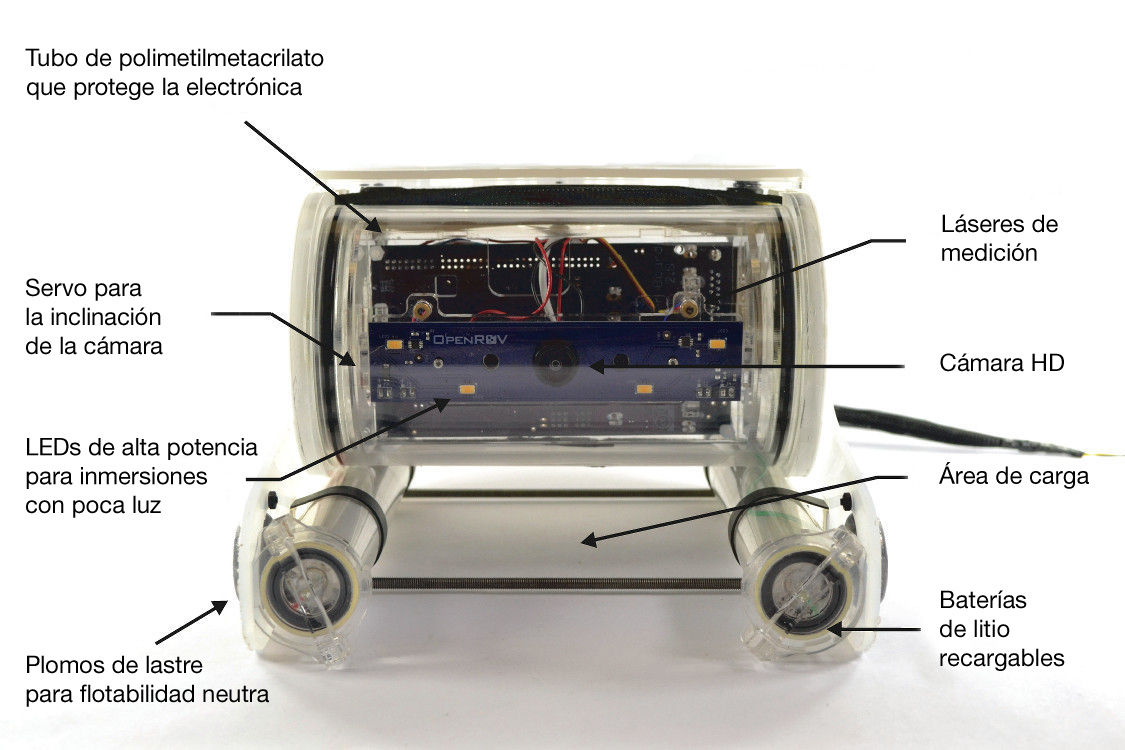
\includegraphics[width=6cm,height=5cm]{img/cap3/ROV_frontal}}
    \subfigure[OpenROV parte trasera]{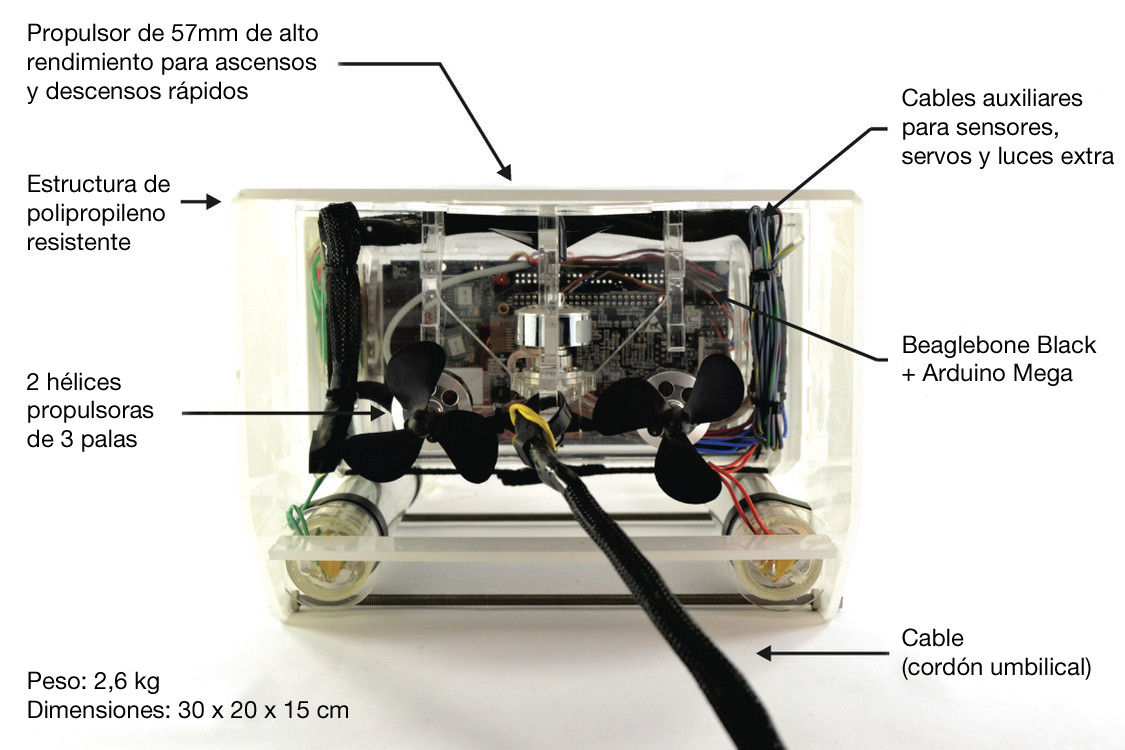
\includegraphics[width=6cm,height=5cm]{img/cap3/ROV_trasera}}
  \end{center}
  \caption{OpenROV}
  \label{fig:ROV-ej}
\end{figure}
\newpage
\section{Estructura y Montaje}
\label{cap:montaje}

En esta sección se va a describir cada paso del montaje del robot, desde el montaje de cada uno de los chasis hasta la electrónica, de la cual tendremos que soldar los elementos.

\subsection{Estructura de OpenROV}
\label{subsec:EstructuraOpenROV}

Antes de comenzar con el montaje de la estructura, la cámara y el chasis del ROV, se necesitarán ciertas herramientas para el correcto ensamblaje.

Las herramientas necesarias son: guantes, gafas, cúter, cemento acrílico y pegamento. Una vez hayamos obtenido todos los materiales empezaremos con el montaje.

\begin{figure} [hbtp]
  \begin{center}
    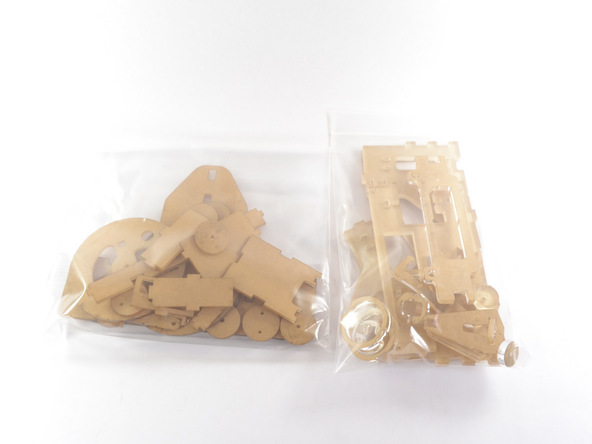
\includegraphics[width=8cm]{img/cap3/3_3/piezas}
  \end{center}
  \caption{Piezas de los chasis.}
  \label{fig:piezas}
\end{figure}

Se separan las piezas para realizar su correcto montaje. Una vez localizadas las piezas para la estructura, se le quitará el papel protector a la pieza. 
Iremos pegando y dejando secar para que se adhiera correctamente. 
Al final, quedará una estructura como la de la imagen.

\begin{figure} [hbtp]
  \begin{center}
    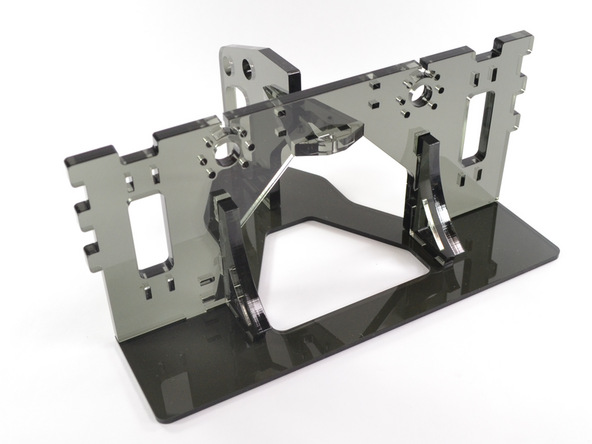
\includegraphics[width=8cm]{img/cap3/3_3/chasis_ppal}
  \end{center}
  \caption{Chasis principal.}
  \label{fig:chasis_ppal}
\end{figure}

Para el montaje de la estructura del soporte de la cámara y el chasis de la electrónica se realizará el mismo procedimiento que en el caso anterior, con un resultado como el de las siguientes fotos:

\begin{figure}[hbtp]
  \begin{center}
    \subfigure[Soporte de la cámara]{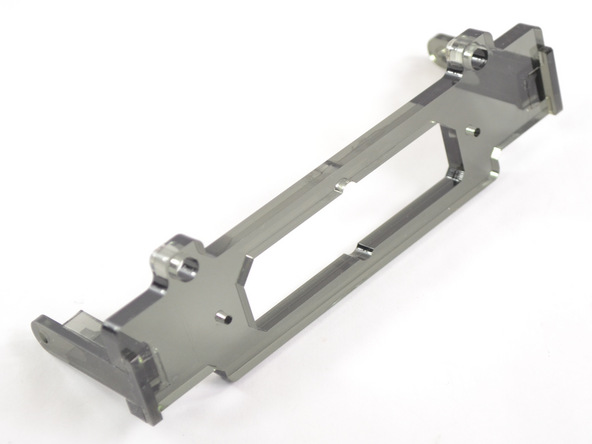
\includegraphics[width=6cm,height=5cm]{img/cap3/3_3/chasis_camara}}
    \subfigure[Chasis de la electrónica]{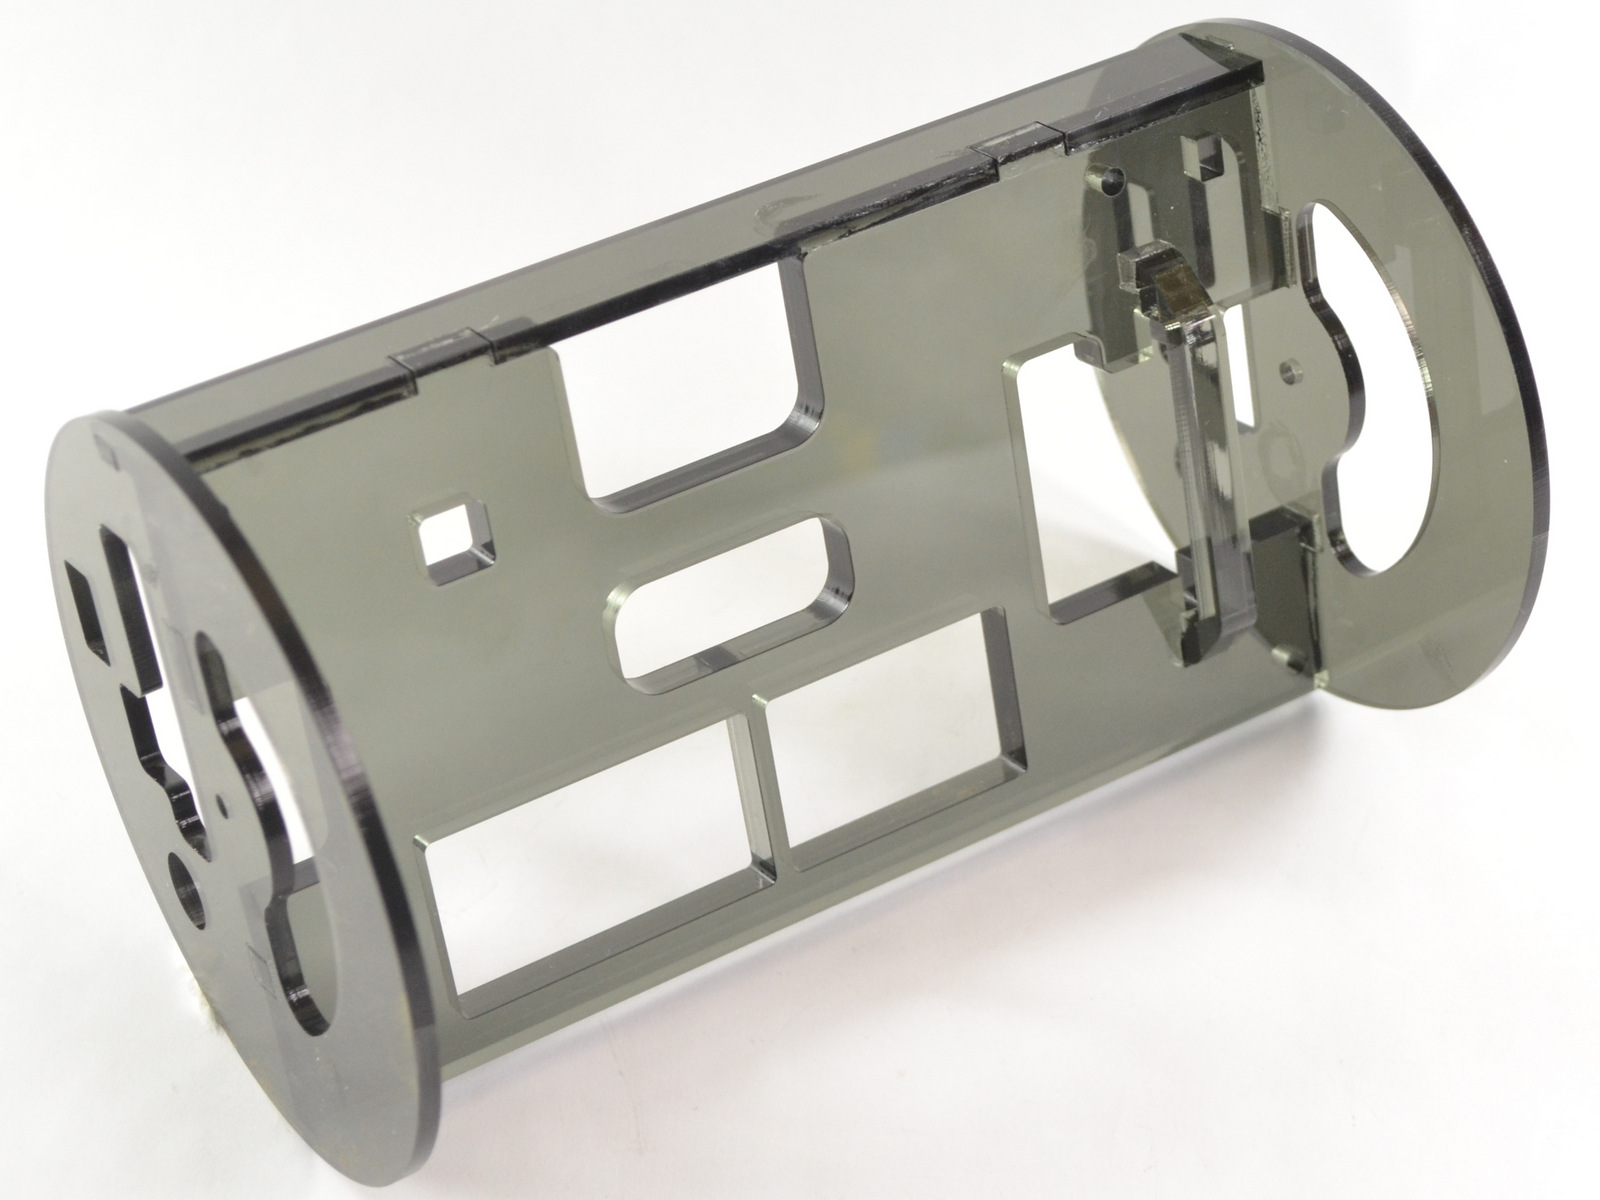
\includegraphics[width=6cm,height=5cm]{img/cap3/3_3/chasis_electronico}}
  \end{center}
  \caption{Soporte de la cámara y electrónica}
  \label{fig:ROV-chasis}
\end{figure}

\subsection{Tapas del chasis}
\label{subsec:tapasChasis}

Al igual  que en el punto anterior, antes de comenzar con el montaje de la tapa, se necesitarán ciertas herramientas para el correcto ensamblaje.

Las herramientas necesarias son: guantes, gafas, cúter, cemento acrílico, SuperGlue y epoxy (epoxy es un tipo de pegamento que soporta estar en contacto con el agua).

En este caso existen dos tapas. En la primera (la superior), necesitaremos una jeringa proporcionada por la comunidad de OpenROV, la cual utilizaremos para preparar la impermeabilización y el sellado de los componentes software del robot.

En la segunda tapa está el conector DB-25, el cual conecta todos los componentes eléctricos. Una vez realizado el montaje de la tapa, se pegará en el espacio sobrante el conector DB-25 y se colocarán los cables adecuadamente en el hueco de la tapa. Cuando esté todo debidamente colocado, se pegará la tapa superior al montaje realizado, lo cual dejará todo debidamente sellado.

\begin{figure}[hbtp]
  \begin{center}
    \subfigure[Tapa inferior desmontada]{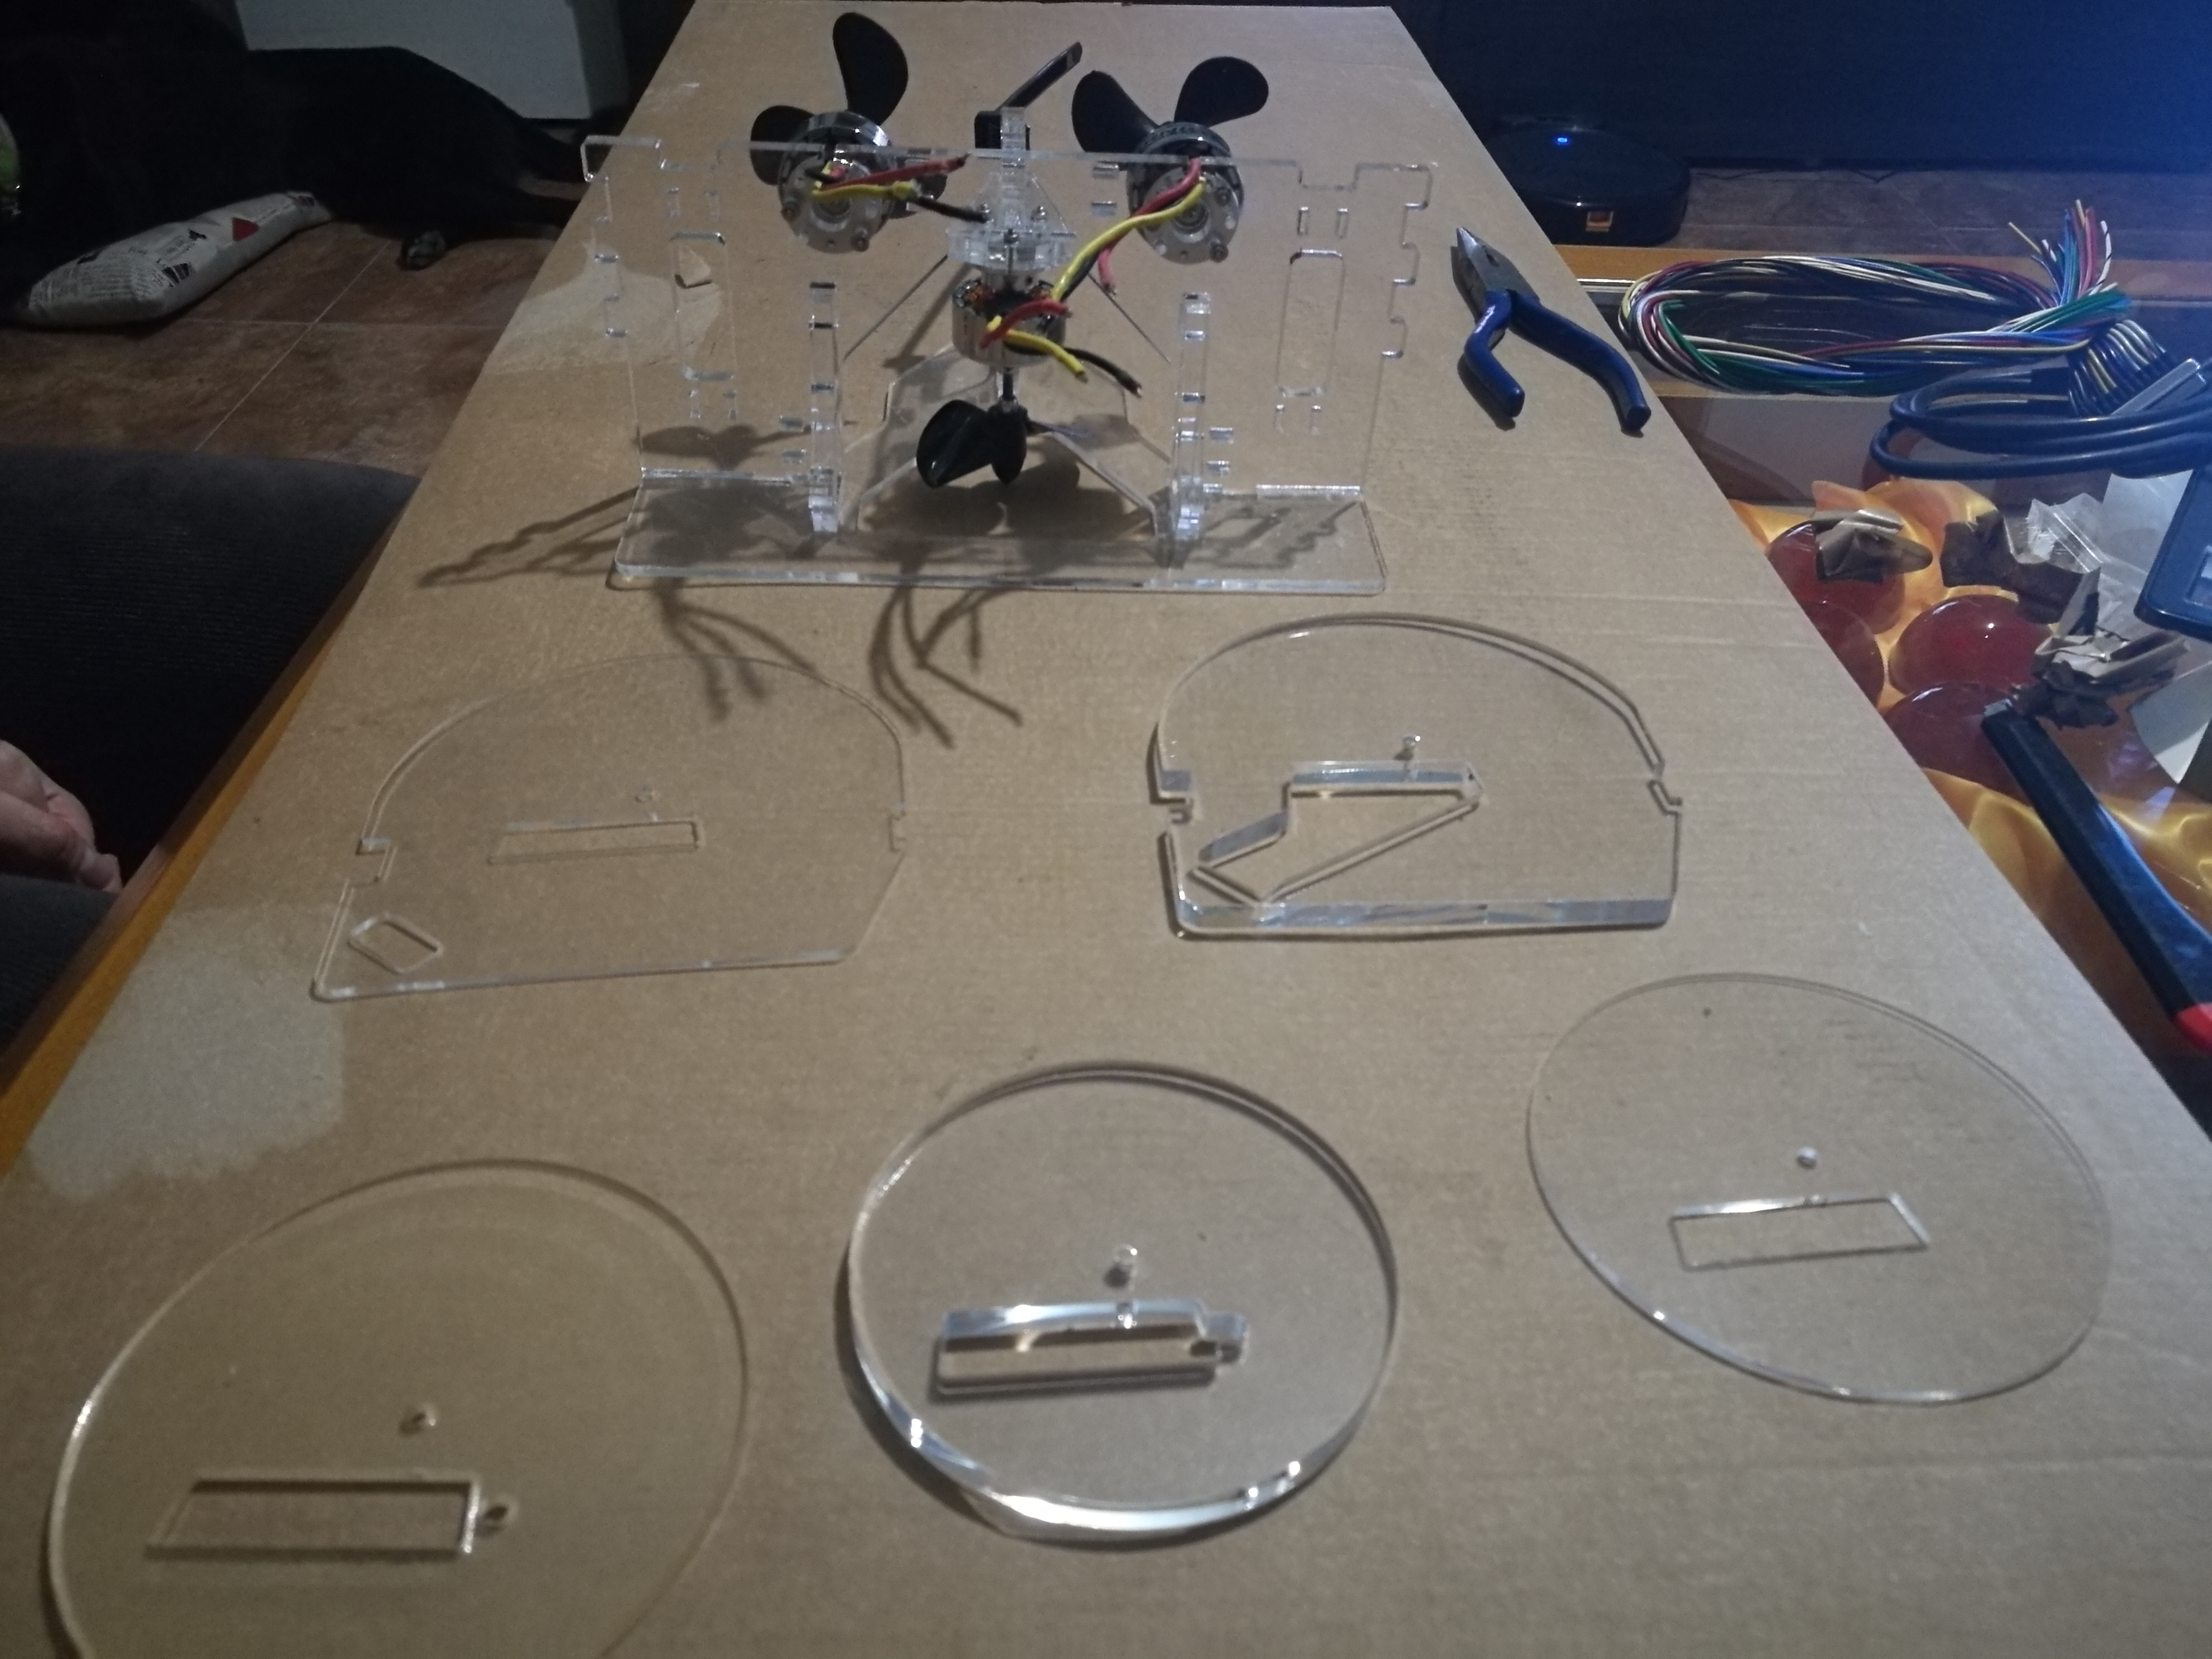
\includegraphics[width=6cm,height=5cm]{img/cap3/3_3/tapa_inf_desmontada}}
    \subfigure[Tapa inferior montada]{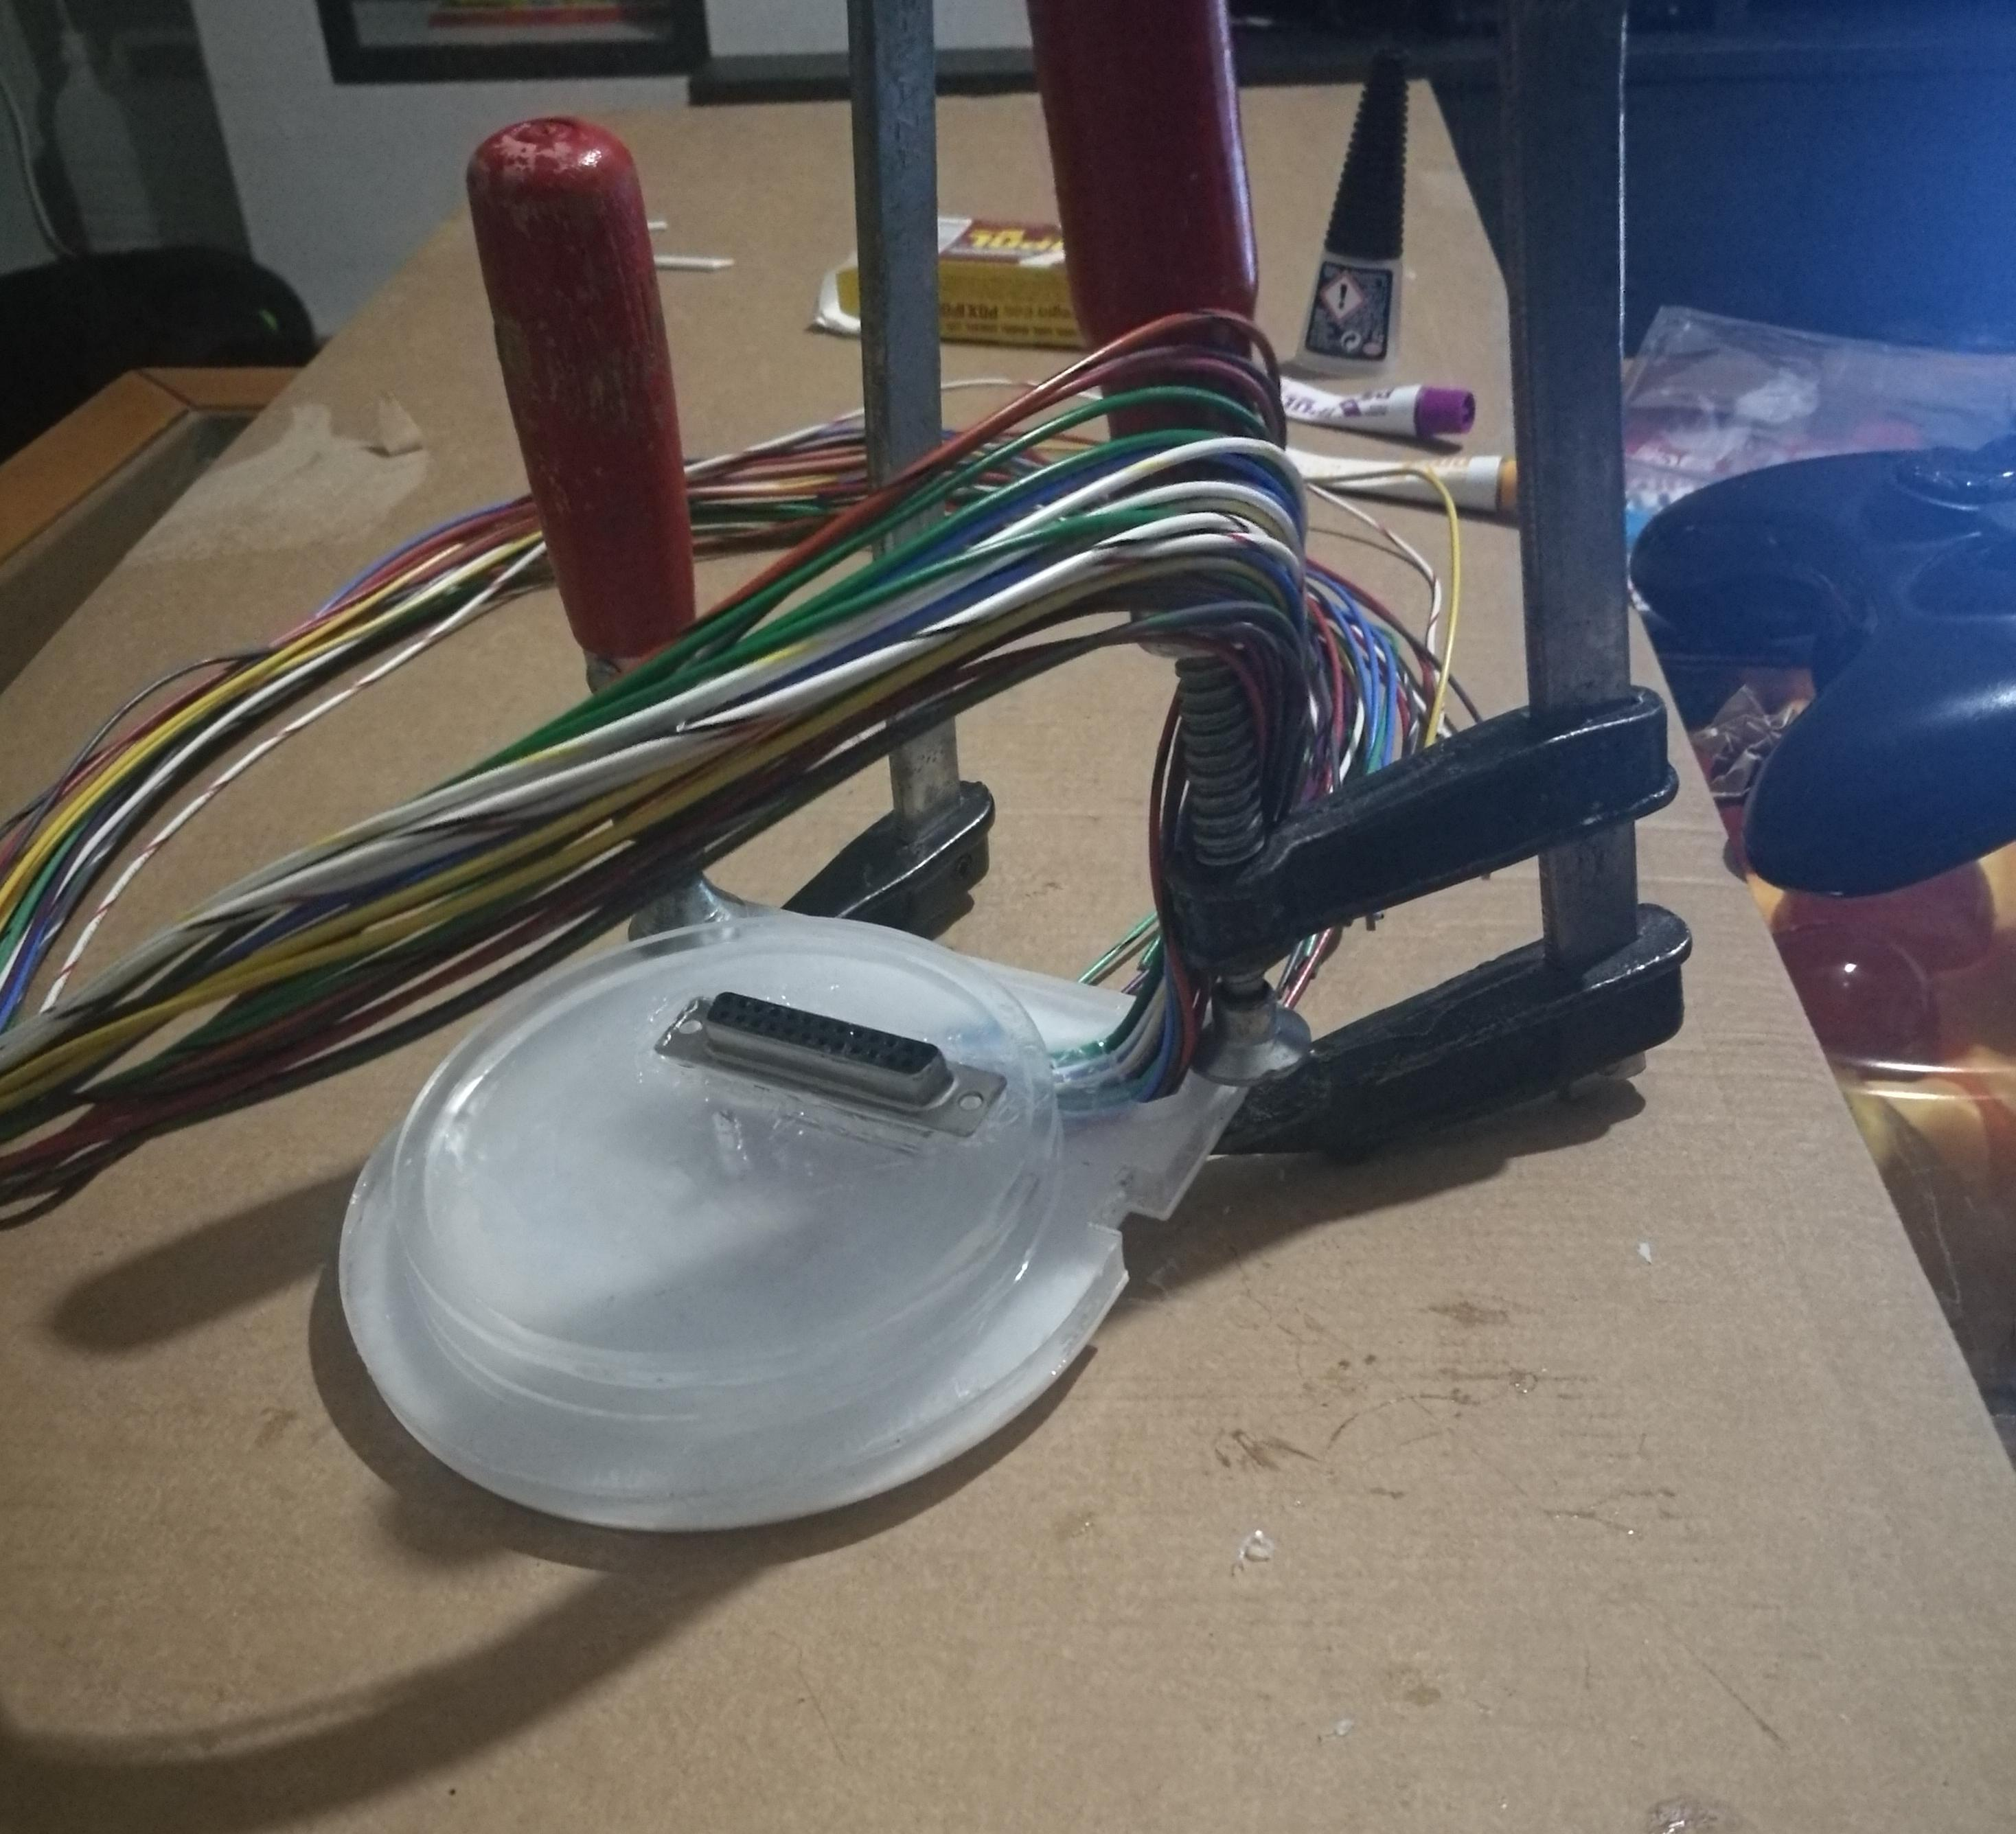
\includegraphics[width=6cm,height=5cm]{img/cap3/3_3/tapa_inf}}
  \end{center}
  \caption{Tapa inferior}
  \label{fig:tapa_iferior}
\end{figure}

\subsection{Electrónica}
\label{subsec:electronica}

Este es el punto crucial del funcionamiento del robot y se necesita especial atención en cada uno de los pasos. 

Al igual que en los apartados anteriores, necesitaremos material especial, entre los que están el soldador, estaño, PLC, BeagleBone, tijeras y destornilladores.

Para empezar, desmontaremos los PLC para sacar el hardware, el cual utilizaremos más adelante.
Uno de los PLC estará interno en el robot, y el otro será el extremo conector que comunicará el ROV con el portátil.

Continuaremos con la placa BeagleBone, que es el procesador principal en el ROV. Funciona junto con un Ardunio para controlar la mayoría de las funciones del ROV.

Una vez juntos el PLC, el BeagleBone y la placa del ROV (Raspberry Pi), constituirán el hardware del robot. Estos elementos se atornillarán para obtener una mejor sujeción. El resultado final lo podemos observar en la siguiente imagen.
\newpage
\begin{figure} [hbtp]
  \begin{center}
    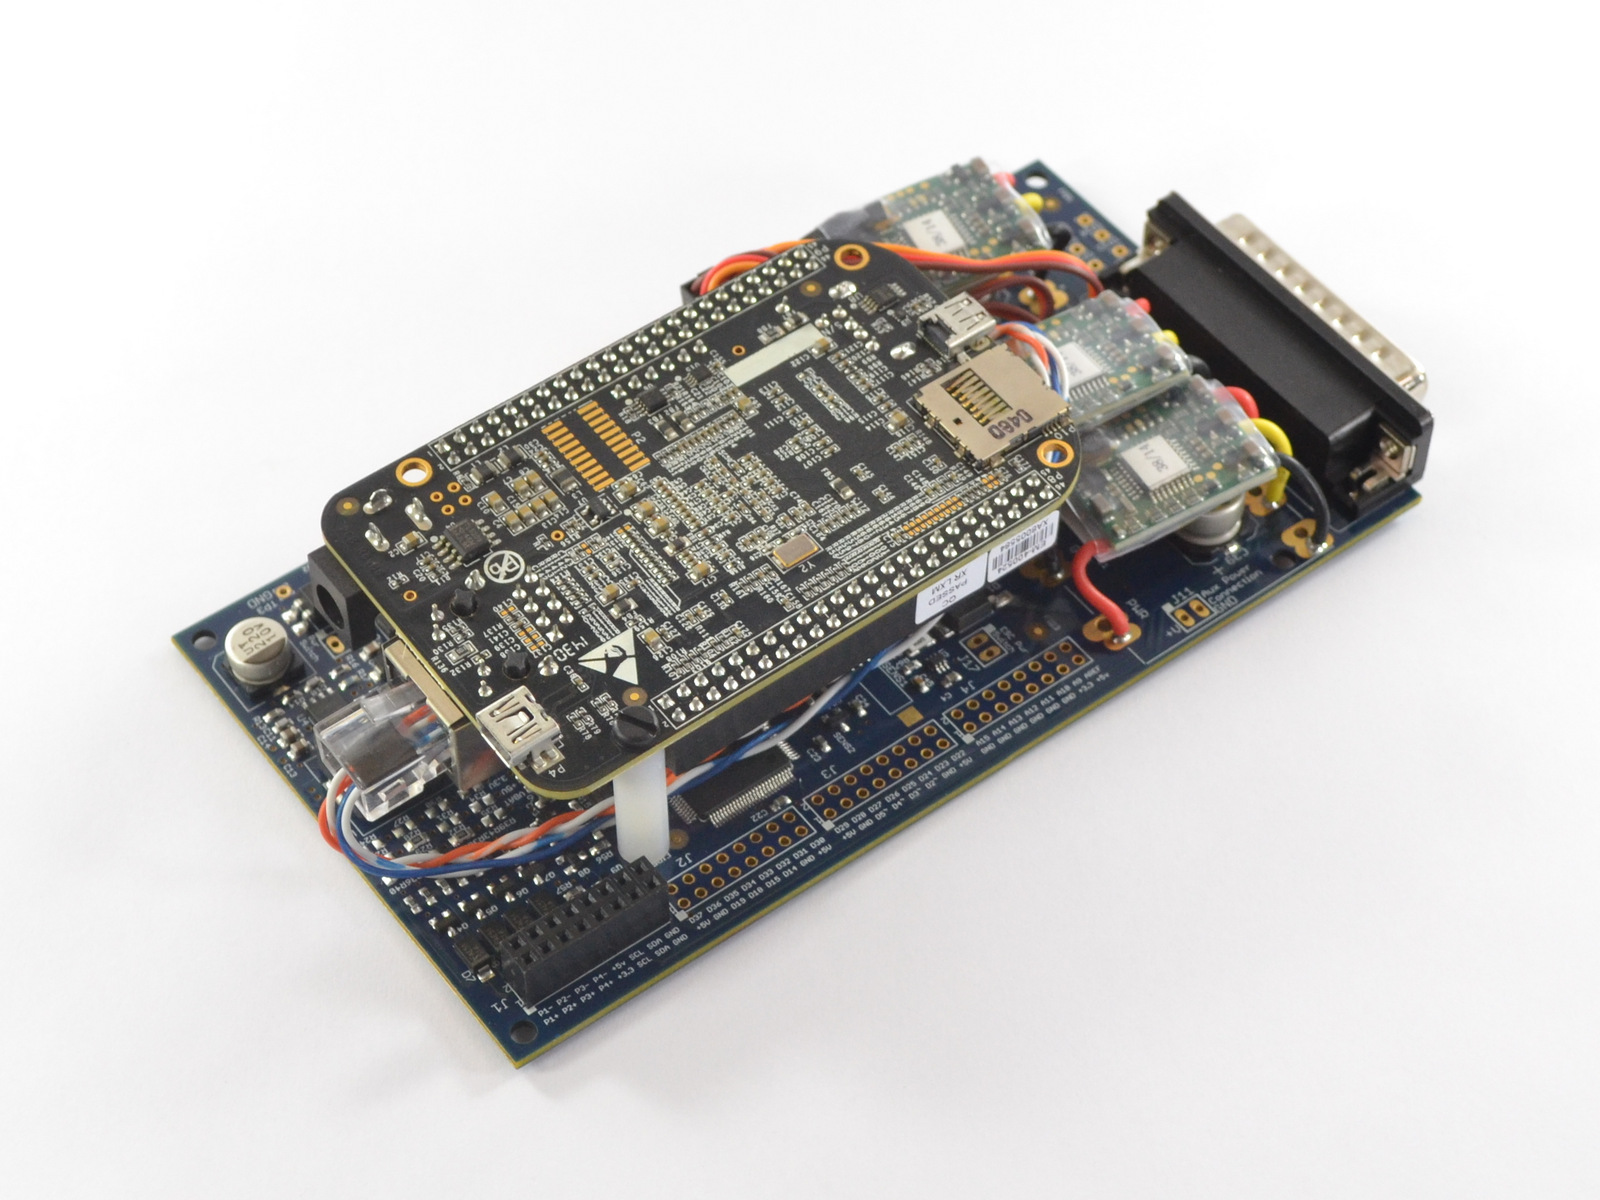
\includegraphics[width=8cm]{img/cap3/3_3/electronica}
  \end{center}
  \caption{Raspberry Pi + PLC + BeagleBone}
  \label{fig:electronica}
\end{figure}

Después, conectaremos el servo al chasis, el cual va a servir para mover la cámara verticalmente.

Continuaremos con la soldadura de los láseres y unos cables a la placa de vídeo del ROV.

\begin{figure} [hbtp]
  \begin{center}
    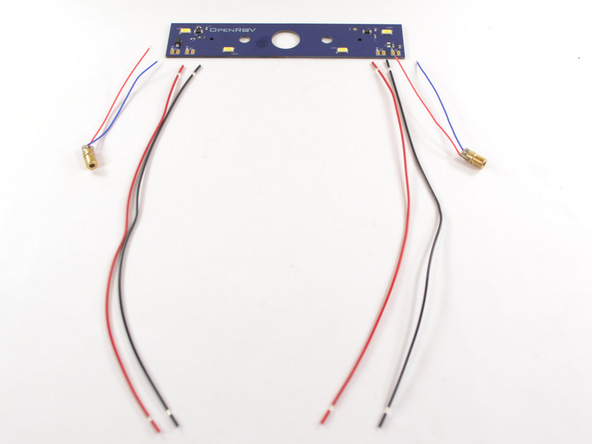
\includegraphics[width=8cm]{img/cap3/3_3/electronica_camara}
  \end{center}
  \caption{Electrónica de la cámara}
  \label{fig:electronica_camara}
\end{figure}

Cuando estén debidamente soldados, se colocará el chasis de la cámara, junto con lo que acabamos de soldar y la cámara. Estos tres elementos los juntaremos con tornillos y tuercas. Para finalizar con este paso, comprobamos que hay un conector al cual enchufaremos un cable que irá directo a la placa principal del ROV.

Para la sujeción de la cámara utilizaremos el chasis principal, que atornillaremos para fijar la cámara. 

Para finalizar este apartado, se conectará el hardware del robot en el lado opuesto de la cámara, y se fijará con tornillos. Se realizará la conexión de los cables a sus ranuras correspondientes.

\subsection{Enrutamiento}
\label{subsec:enrutamiento}

En esta fase se va a requerir unas herramientas más específicas para realizar el montaje, ya que necesitaremos soldar e impermeabilizar con una pistola de calor, además, de tijeras, epoxy, super Glue y bridas.

Empezaremos calculando la distancia de los cables y separaremos los de color verde claro y naranja, para la conexión de las baterías. Los cables verdes oscuros, rojos y azules, los utilizaremos para el montaje de los servomotores. Iremos fijando los cables con las bridas para una correcta colocación.

Cada uno de los tres motores servo lleva tres cables, los cuales soldaremos con los cables correspondientes. Una vez soldados con una silicona especial, se rellenará el espacio del cable soldado y con la pistola de calor se fijará e impermeabilizará. Podemos ver parte del proceso en la siguiente imagen.

%\newpage

\begin{figure} [hbtp]
  \begin{center}
    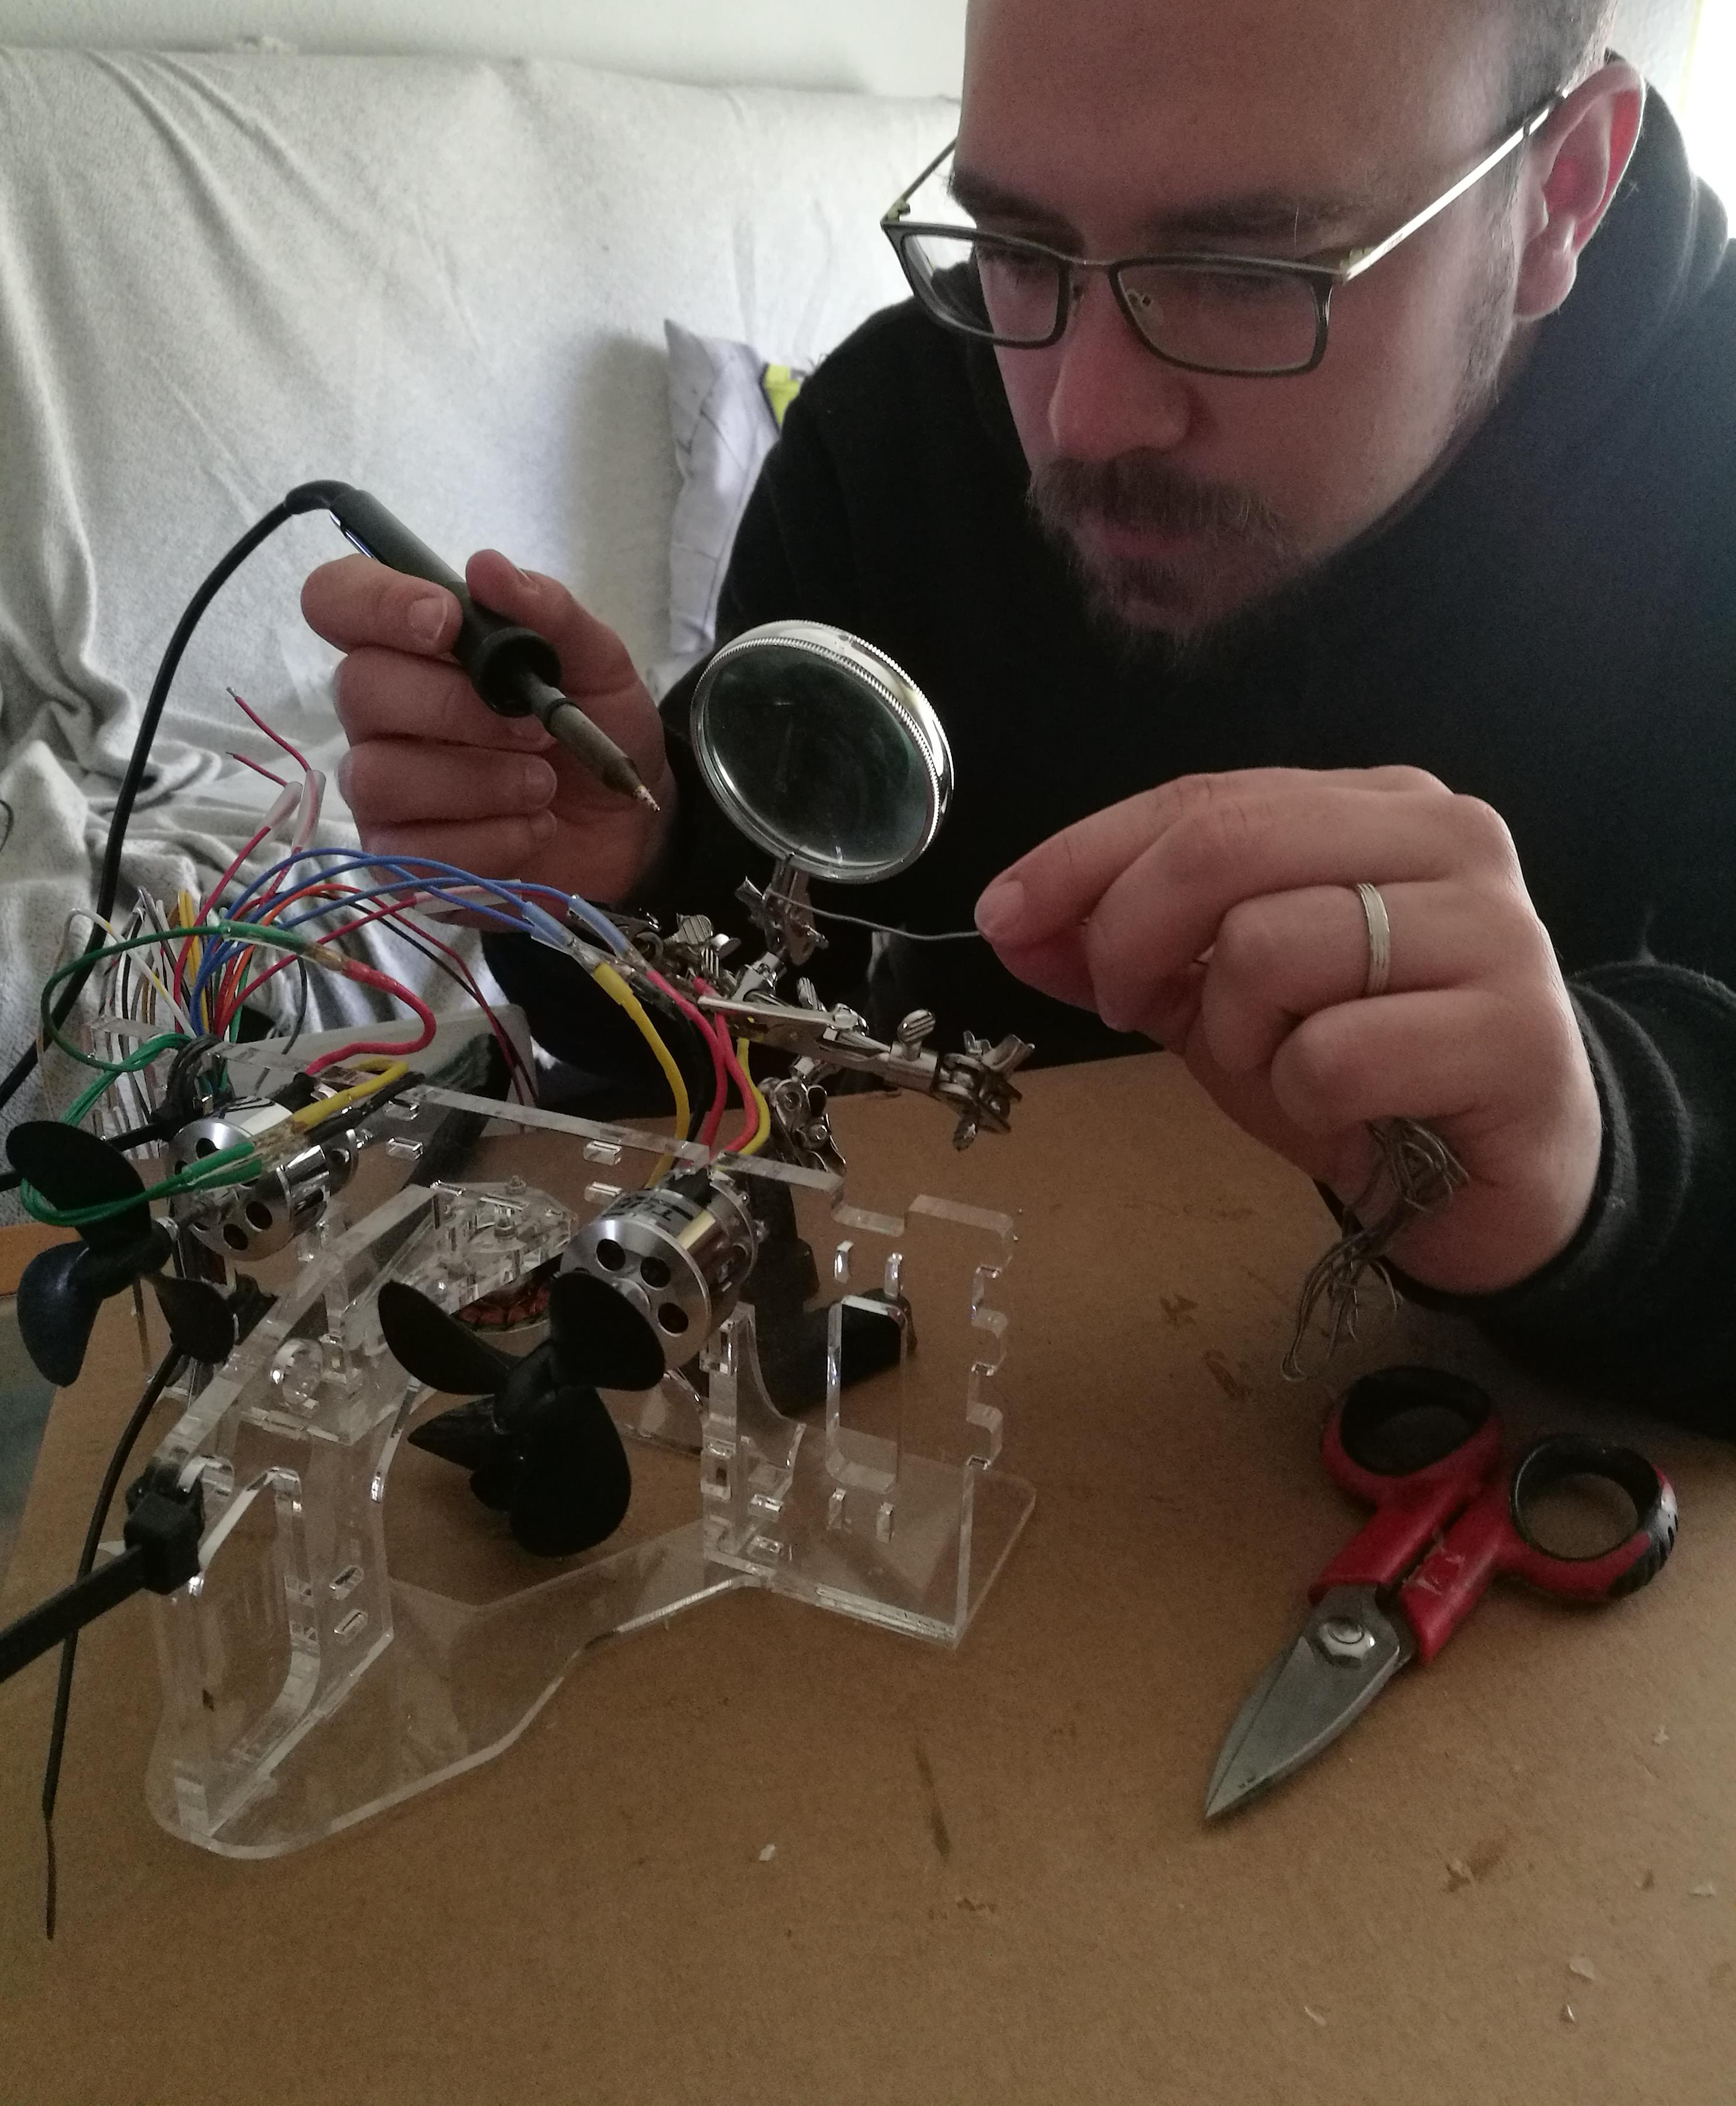
\includegraphics[width=5cm]{img/cap3/3_3/soldar}
  \end{center}
  \caption{Soldadura de cables}
  \label{fig:soldar}
\end{figure}

Continuaremos con el montaje de los dos tubos de la batería. Primero, necesitaremos realizar el montaje de las piezas y soldaremos el muelle (borne) con un chip facilitado por la comunidad de ROV. Esta será la parte negativa de las baterías.
En el extremo del cable sobrante, se rellenará con estaño y se soldará al cable formando la parte positiva, en la que irá conectada la batería.

\subsection{Final}
\label{subsec:final}

En la parte final del montaje será necesaria una soldadura con el cable de par trenzado, que es el encargado de mandar la señal al portátil.

El otro extremo del cable de par trenzado irá conectado al PLC. Gracias a este cable, el robot puede sumergirse a una distancia de 100 m. Usaremos una brida de mayor tamaño para fijar el cable y así obtener una mayor seguridad, ya que si el robot quedara expuesto a un problema en la inmersión, es probable que necesitemos tirar de él.

En el cuerpo principal del robot, con unas gomas, sujetaremos los tubos que llevarán las baterías y fijaremos los extremos con dos varillas de metal.
\\Para aislar el hardware se usará un tubo cilíndrico trasparente de polimetilmetacrilato previamente limado en los extremos.
\\Cuando todo el montaje esté terminado, pondremos más seguridad al hardware, añadiendo una cuerda que hará presión.

Además, colocaremos dos pesas de 300 g en los brazos del ROV para que la sumersión sea más fácil y fiable.

\section{Conectividad OpenROV}
\label{cap:Conectividad OpenROV}
  
En esta sección se marcarán las pautas necesarias para realizar el correcto funcionamiento del software del OpenROV.  
  
\subsection{Diseño de Conectividad}
\label{subsec:disenio}

Para encender el ROV, necesitaremos el cable mini USB y el cable ethernet debidamente colocado en el extremo del PLC y estos a su vez al portátil.

\begin{figure} [hbtp]
\begin{center}
  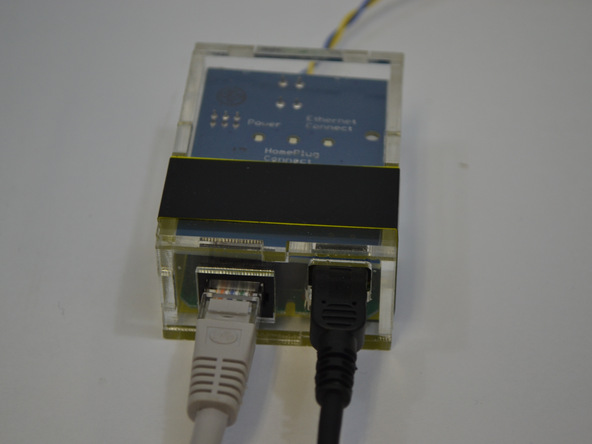
\includegraphics[width=8cm]{img/cap3/3_4/plc_externo}
\end{center}
\caption{PLC externo}
\label{fig:plc_ext}
\end{figure}

\newpage
El conector USB actúa como interruptor de encendido/apagado del robot.

El ROV tiene una dirección IP estática 192.168.254.1. Para conectarnos a la web del robot, la dirección ethernet de nuestro ordenador debe pertenecer a la misma subred, es decir, 192.168.254.2. La máscara de subred se establece en la dirección 255.255.255.0.

Pero para poder mostrar la página, antes debemos realizar una serie de pasos, en la que necesitaremos una tarjeta microSD para realizar la configuración del ROV.
  
\begin{enumerate}
\item Se descarga la imagen más reciente de OpenROV 2.8, en este caso, la versión es 30.0.3. Una vez descargado se descomprime el archivo .zip, dejando en el directorio de descarga un fichero con la extensión .img.
\item Formateamos la tarjeta microSD y montamos la imagen descargada en la tarjeta. Una vez terminado el proceso, quitamos la tarjeta del portátil.
\item Conectamos la tarjeta microSD al BeagleBone, y conectamos el ROV con el cable USB para encenderlo. Los LED de la placa BeagleBone parpadearán para mostrar que la imagen se está aplicando a la memoria de la placa. El proceso terminará cuando los cuatro leds estén encendidos. Si pasado un tiempo no lucen los cuatro leds, habría que repetir este punto.

Cuando esté completo, retiraremos el cable USB del portátil para desconectar el ROV y retiraremos la tarjeta microSD de la placa BeagleBone.

Terminado este proceso, volveremos a conectar la tarjeta en el portátil.

\begin{figure} [hbtp]
\begin{center}
  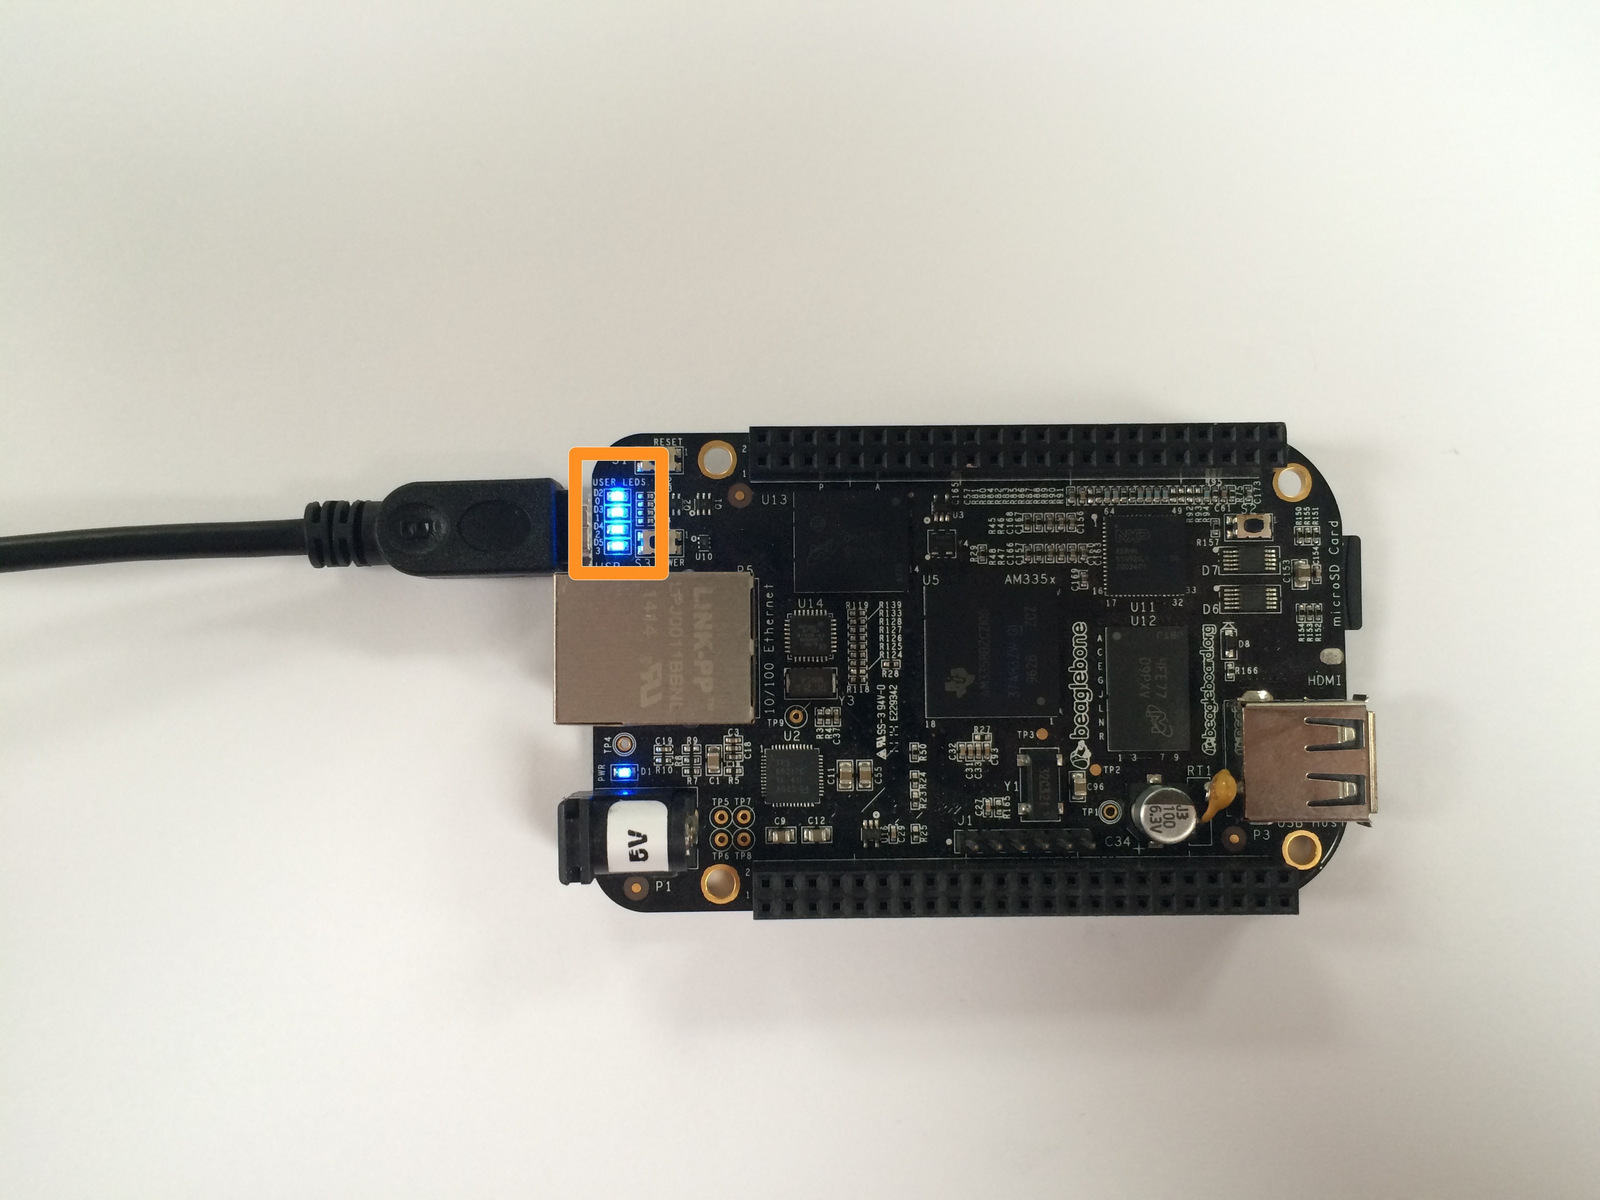
\includegraphics[width=8cm]{img/cap3/3_4/BBB}
\end{center}
\caption{BeagleBone configurada}
\label{fig:bbb}
\end{figure}
\item Como se mencionó al principio del apartado, el ROV tiene una dirección IP estática incorporada de 192.168.254.1. Para conectarnos, configuraremos nuestro ordenador con la dirección IP 192.168.254.2 y con la máscara de subred en la dirección 255.255.255.0.

En Windows 8 la configuración sería:

\renewcommand{\lstlistingname}{Configuración}
\begin{lstlisting}[caption= Windows 8, label={lst:config_w8}]
Ir al Panel de control.
Seleccionar Red e Internet.
Ir a red y centro compartido, pulsar cambiar configuracion de adaptador y marcar la opcion de ethernet.
En propiedades usamos la direccion IP 192.168.254.2
\end{lstlisting}

\begin{figure} [hbtp]
\begin{center}
  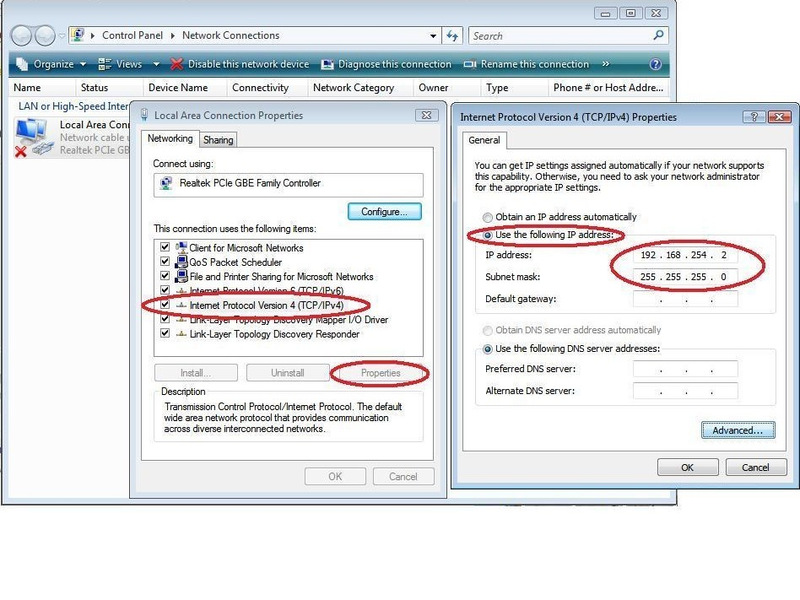
\includegraphics[width=10cm]{img/cap3/3_4/conexion}
\end{center}
\caption{Conexión Windows 8}
\label{fig:w8}
\end{figure}

En Ubuntu la configuración de una nueva IP estática sería:

\renewcommand{\lstlistingname}{Configuración}
\begin{lstlisting}[caption= Ubuntu, label={lst:config_ubuntu}]
  # Abrir el terminal (Ctrl + Atl + T).
  # Comprobamos las interfaces del equipo:  
  $ ifconfig -a
  # Editamos el archivo de configuracion de las interfaces:  
  $ sudo vim /etc/network/interfaces

  # Configuracion de direccion IP fija para el interfaz eth0
    auto eth0
    iface eth0 inet static
    address 192.168.254.2
    netmask 255.255.255.0
    network 192.168.254.0
    broadcast 192.168.254.255
    gateway 192.168.254.1
\end{lstlisting}

  Donde:
    \subsubitem address es la dirección IP que quieres ponerle a tu máquina.
    \subsubitem netmask es la máscara de subred de esa dirección IP.
    \subsubitem network es la red a la que pertenece esa dirección IP.
    \subsubitem broadcast es la direción IP de difusión de esa red.
    \subsubitem gateway es la dirección IP de la puerta de enlace predeterminada.

\subitem Reiniciamos las interfaces de red para aplicar los cambios:

\renewcommand{\lstlistingname}{}
\begin{lstlisting}[caption=Reinicio, label={lst:reset}]
  $ sudo /etc/init.d/networking restart
\end{lstlisting}
\item Abriremos el navegador Google-Chrome, y en la barra de direcciones escribiremos la IP 192.168.254.1:8080, que es la dirección IP de OpenROV. Accederemos a la web, que es la interfaz de OpenROV.
\item Para finalizar, deberemos actualizar el firmware en la web, presionaremos el botón de configuración en la parte superior derecha de la pantalla y presionaremos “Cargar firmware desde la tarjeta SD a Ardruino”.
La tarjeta microSD no debe estar en el ROV. Presionaremos “Mostrar Detalles” y seguidamente, “Aplicar nuevo Firmware”.
Una vez que la carga sea exitosa, como se muestra en la imagen, se retirará el cable USB del portátil para desconectar el ROV. Volveremos a conectar el cable USB al portátil para realizar el reinicio.


\begin{figure} [hbtp]
\begin{center}
  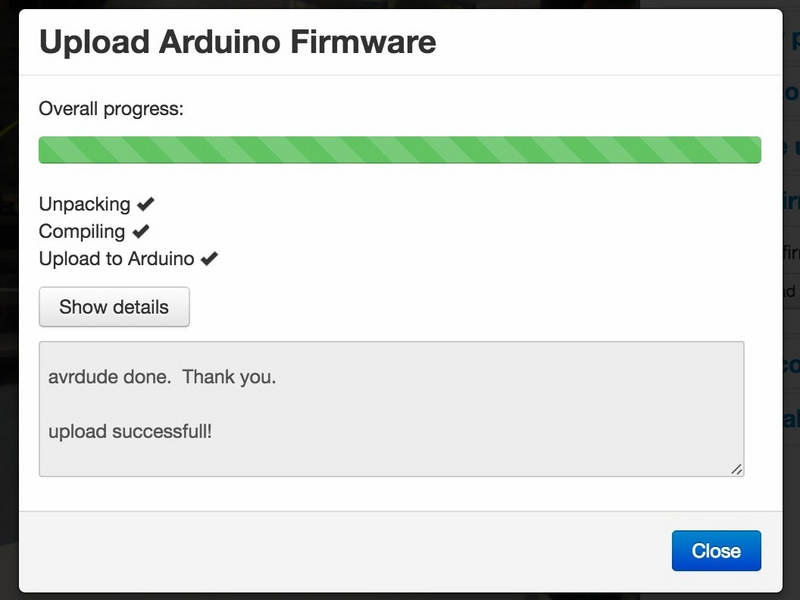
\includegraphics[width=8cm]{img/cap3/3_4/firmware}
\end{center}
\caption{Actualización firmware}
\label{fig:firmware}
\end{figure}

\end{enumerate}
  
  
  
\subsection{Puesta a punto de los elementos}
\label{subsec:elementos}
  \subsubsection{Cámara}
  \label{subsubsec:camara}
Ajustaremos el foco de la lente de la cámara hasta que la imagen pueda verse con nitidez.
\begin{figure} [hbtp]
\begin{center}
  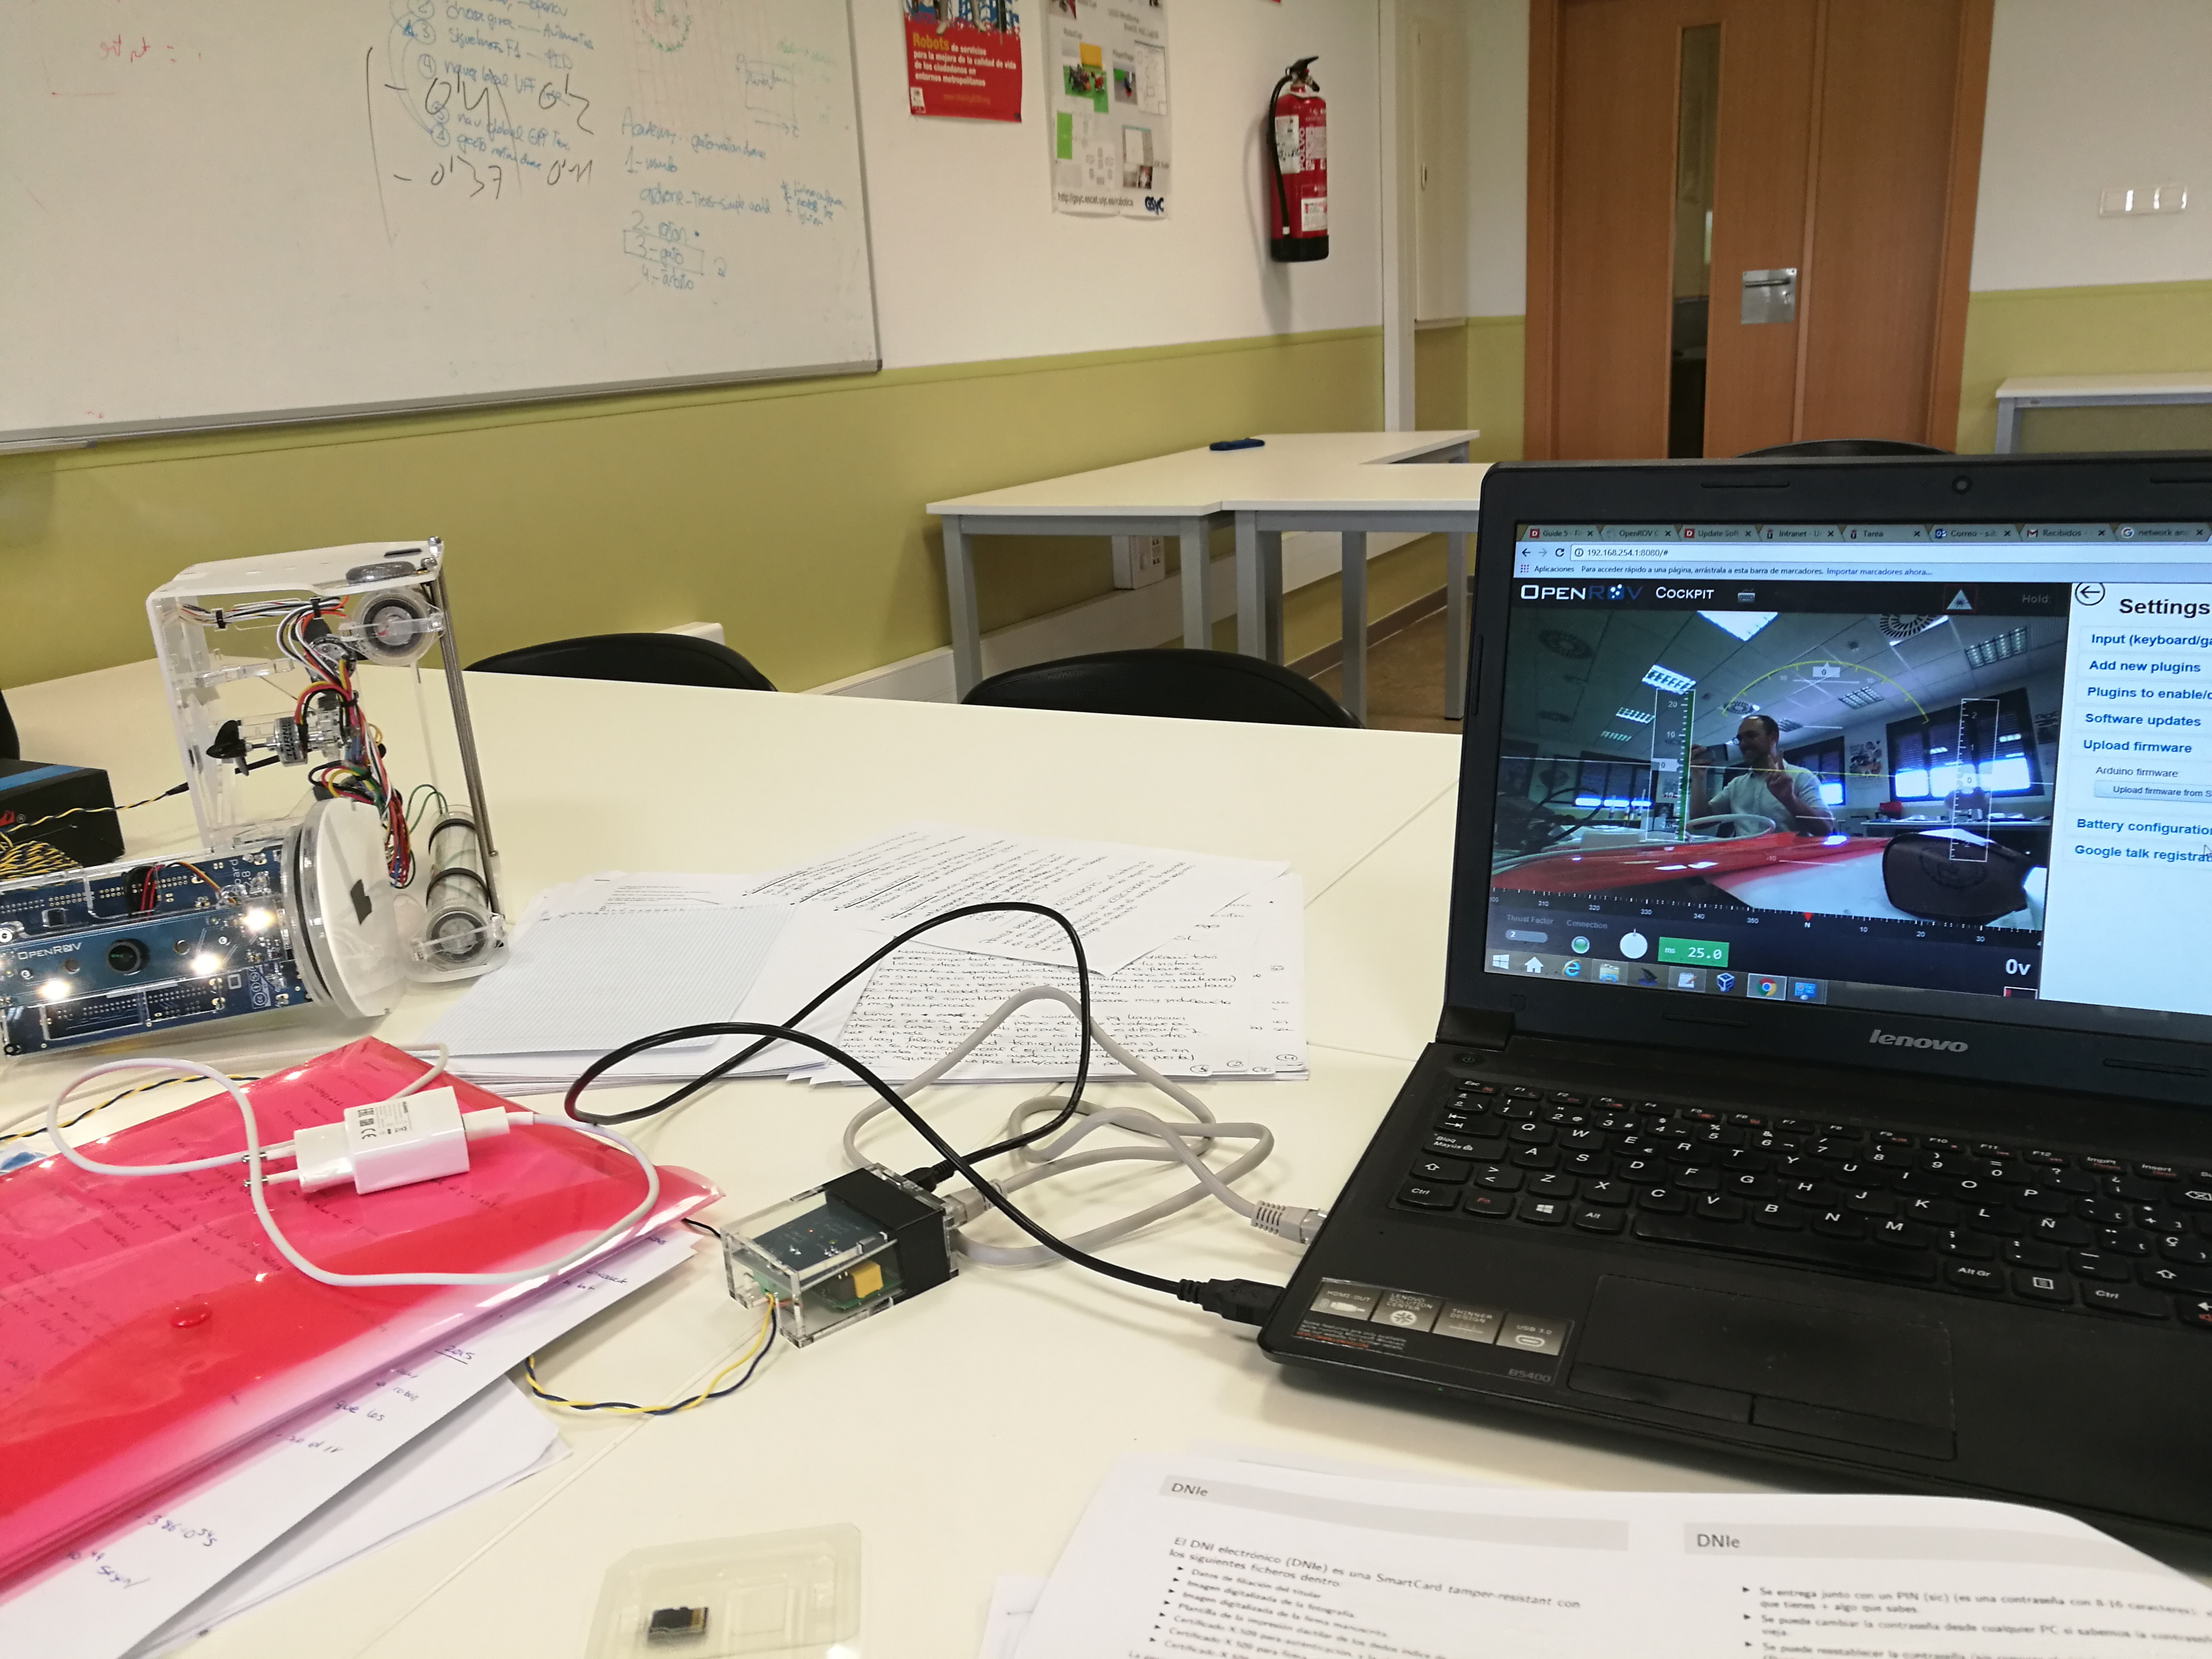
\includegraphics[width=8cm]{img/cap3/3_4/foco}
\end{center}
\caption{Foco cámara}
\label{fig:foco}
\end{figure}
    
  \subsubsection{Láser}
  \label{subsubsec:laser}
El ROV lleva incorporado dos láseres, que hemos soldado previamente a la placa de la cámara. El proceso que llevaremos a cabo será su calibración y pegado en el chasis.
En un papel dibujaremos dos “X” separadas entre sí diez centímetros, y colocaremos esa hoja a una distancia de entre tres y cuatro metros del robot, el cual debe estar a la misma altura que el folio.
Si pesionamos la tecla L en la web, encenderemos los láseres. Para apagarlos, simplemente hay que volver a pulsar la tecla L.
Una vez esté todo calibrado, pegaremos con Super Glue los láseres al chasis de la cámara.
 \begin{figure}[hbtp]
  \begin{center}
    \subfigure[Distancia de los láseres]{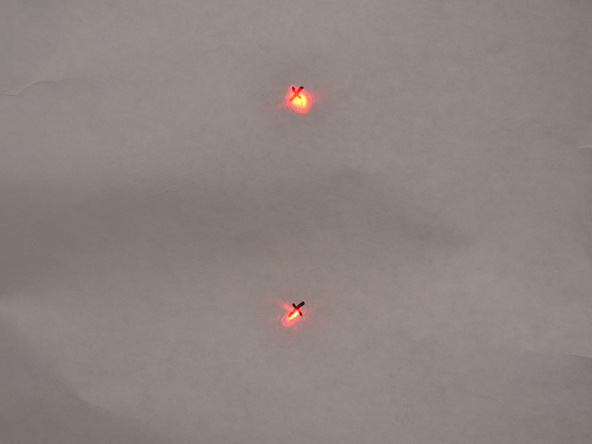
\includegraphics[width=6cm,height=5cm]{img/cap3/3_4/laseres}}
    \subfigure[Fijado del los láseres]{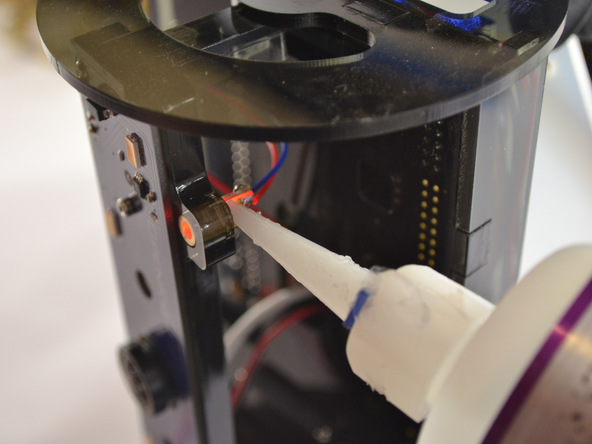
\includegraphics[width=6cm,height=5cm]{img/cap3/3_4/laser_camara}}
  \end{center}
  \caption{Láser}
  \label{fig:laser}
\end{figure}

\newpage
\subsubsection{Motores}
\label{subsubsec:motores}
En este punto se realizará una comprobación de las hélices. Para ver si su rotación es la correcta, presionaremos la tecla de “flecha arriba”, y observaremos en qué dirección giran los motores.
El motor izquierdo (amarillo) debe funcionar en sentido contrario a las agujas del reloj.
El motor derecho (azul) debe funcionar en sentido a las agujas del reloj.
\begin{figure} [hbtp]
\begin{center}
  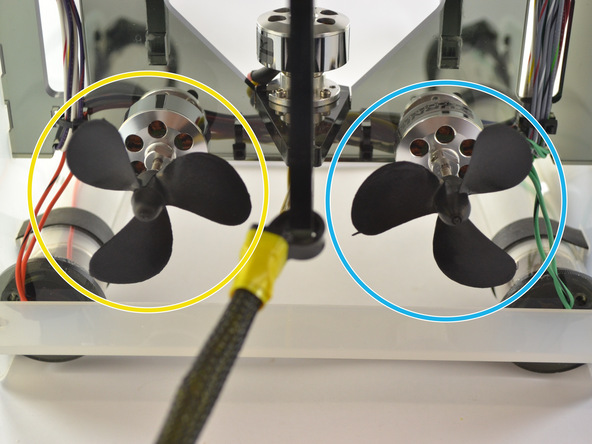
\includegraphics[width=8cm]{img/cap3/3_4/motores}
\end{center}
\caption{Motores}
\label{fig:motores}
\end{figure}

Si el giro es incorrecto, invertiremos su rotación en la parte de “diagnóstico” de la web. Seleccionaremos la opción “invertir” del motor o motores que queramos modificar.

\begin{figure} [hbtp]
\begin{center}
  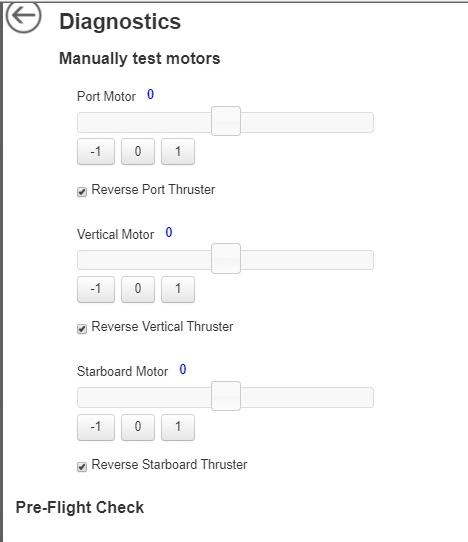
\includegraphics[width=7cm]{img/cap3/3_4/diagnostic}
\end{center}
\caption{Diagnóstico}
\label{fig:diagnostics}
\end{figure} 

\newpage
\subsubsection{Tubo cilíndrico trasparente de polimetilmetacrilato}
\label{subsubsec:tubo}
El tubo cilíndrico contendrá todo el sistema hardware y software del ROV.
Para una mejor fijación, lijaremos los bordes interiores para que la junta se ajuste al tubo.
\begin{figure} [hbtp]
\begin{center}
  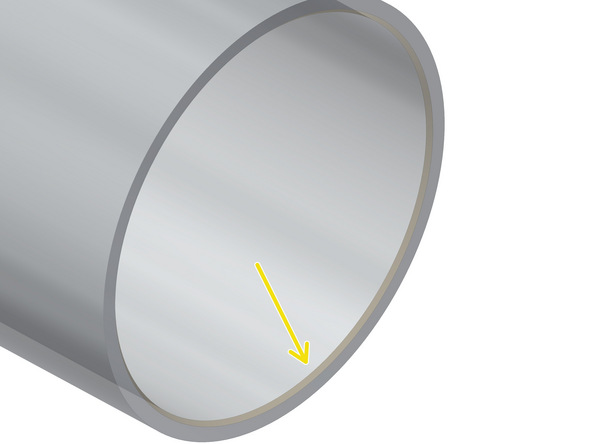
\includegraphics[width=8cm]{img/cap3/3_4/tubo}
\end{center}
\caption{Tubo}
\label{fig:tubo}
\end{figure}

\subsubsection{Tapa superior}
\label{subsubsec:tapa}
Una vez instalado el tubo, verificaremos que la junta esté bien introducida a lo largo de todo el perímetro interior del tubo.
La tapa superior contiene un orificio de ventilación para igualar la presión al colocar las tapas.
\begin{figure} [hbtp]
\begin{center}
  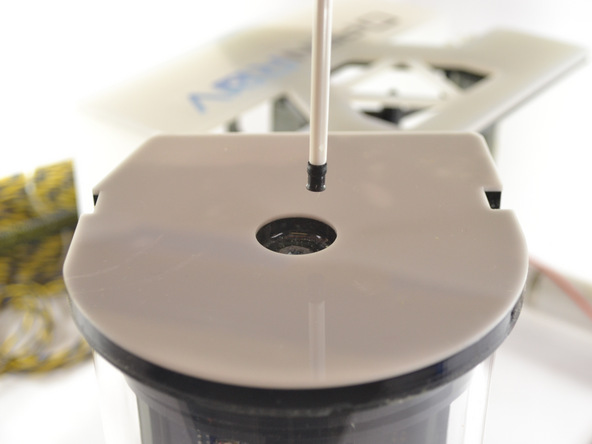
\includegraphics[width=8cm]{img/cap3/3_4/tapa_superior}
\end{center}
\caption{Tapa superior}
\label{fig:tapa_sup}
\end{figure}  

\newpage
\subsection{Web/Cockpit}
\label{subsec:cockpit}
El manejo del ROV se consigue gracias a la web Cockpit, que es la interfaz de usuario y contiene todos los sistemas de control de cualquier vehículo o dispositivo operado a distancia.

\begin{figure} [hbtp]
\begin{center}
  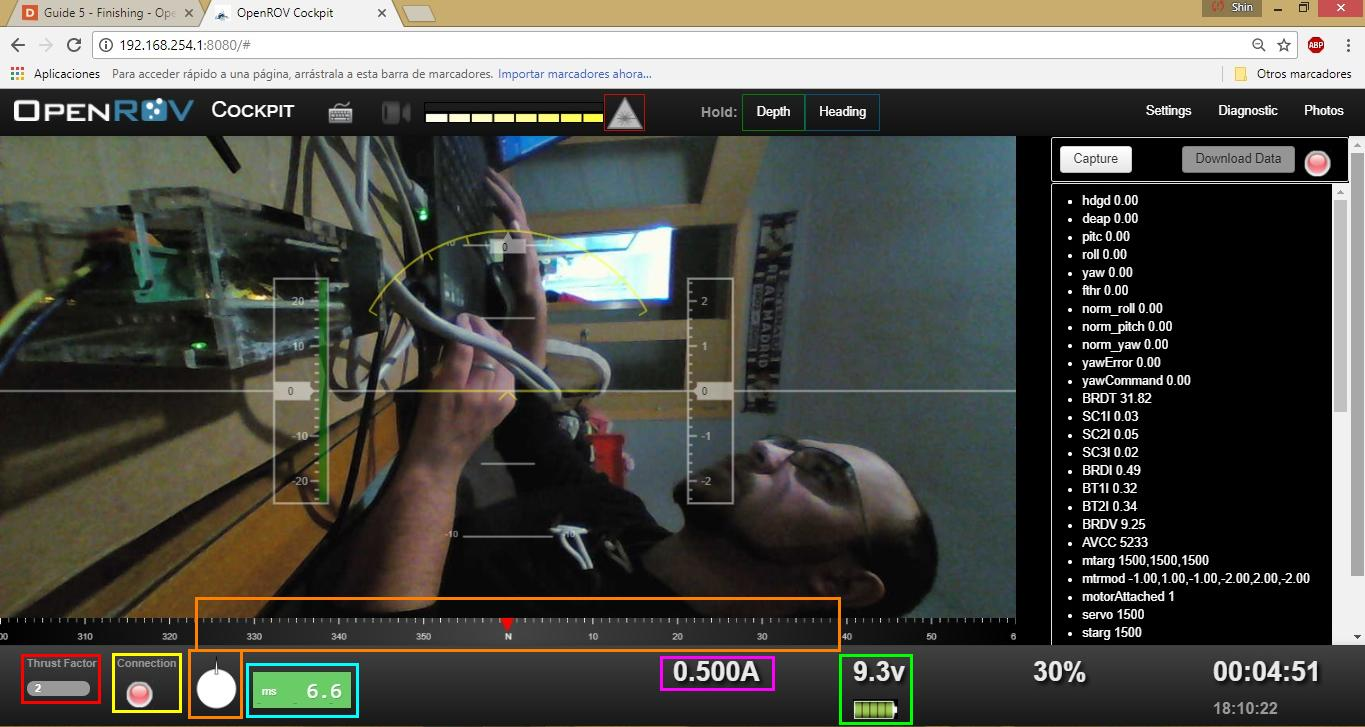
\includegraphics[width=15cm]{img/cap3/3_5/cockpit1_v2}
\end{center}
\caption{Cockpit (1)}
\label{fig:cockpit1}
\end{figure}

\begin{itemize}
\item[\textcolor{red}{\textbullet}]Configuración de potencia de los motores (1, la más baja y 5, la más alta).
\item[\textcolor{yellow}{\textbullet}]Conectividad (verde = conectado).
\item[\textcolor{orange}{\textbullet}]Brújula.
\item[\textcolor{blue}{\textbullet}]Latencia (si hubiera algún problema mostraría +999).
\item[\textcolor{purple}{\textbullet}]Intensidad de corriente los componentes electrónicos en Amperios.
\item[\textcolor{green}{\textbullet}]Potencia de las baterías.
\end{itemize}

\begin{figure} [hbtp]
\begin{center}
  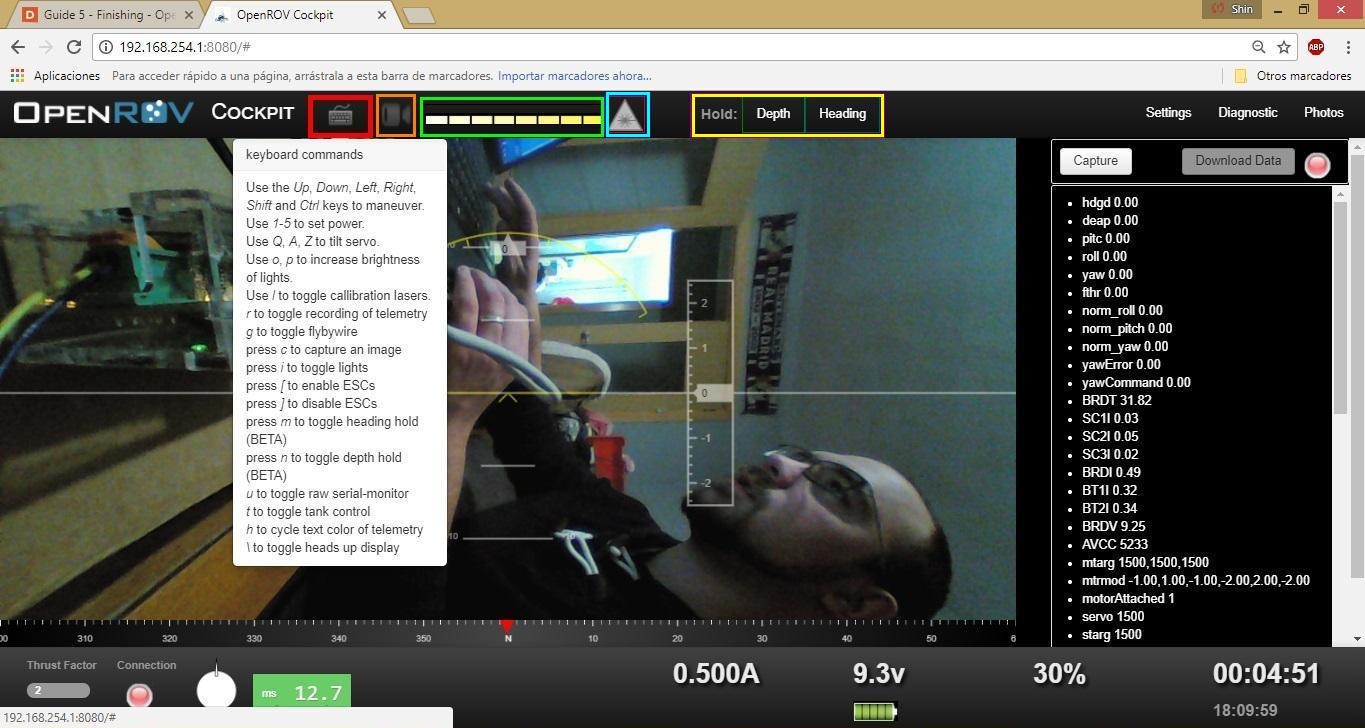
\includegraphics[width=15cm]{img/cap3/3_5/cockpit2_v2}
\end{center}
\caption{Cockpit (2)}
\label{fig:cockpit2}
\end{figure}

\begin{itemize}
\item[\textcolor{red}{\textbullet}]Pulsando el botón señalado en rojo (el icono del teclado) se obtienen los comandos de uso del robot.
\item[\textcolor{orange}{\textbullet}]Indicador de la cámara.
\item[\textcolor{green}{\textbullet}]Indicador de nivel de luz.
\item[\textcolor{blue}{\textbullet}]Indicador de encendido/apagado del láser.
\item[\textcolor{yellow}{\textbullet}]Indicadores de profundidad y rumbo. Se alternan entre encendido/apagado para mantener la profundidad actual y/o el rumbo.
\end{itemize}


\newpage
\begin{figure} [hbtp]
\begin{center}
  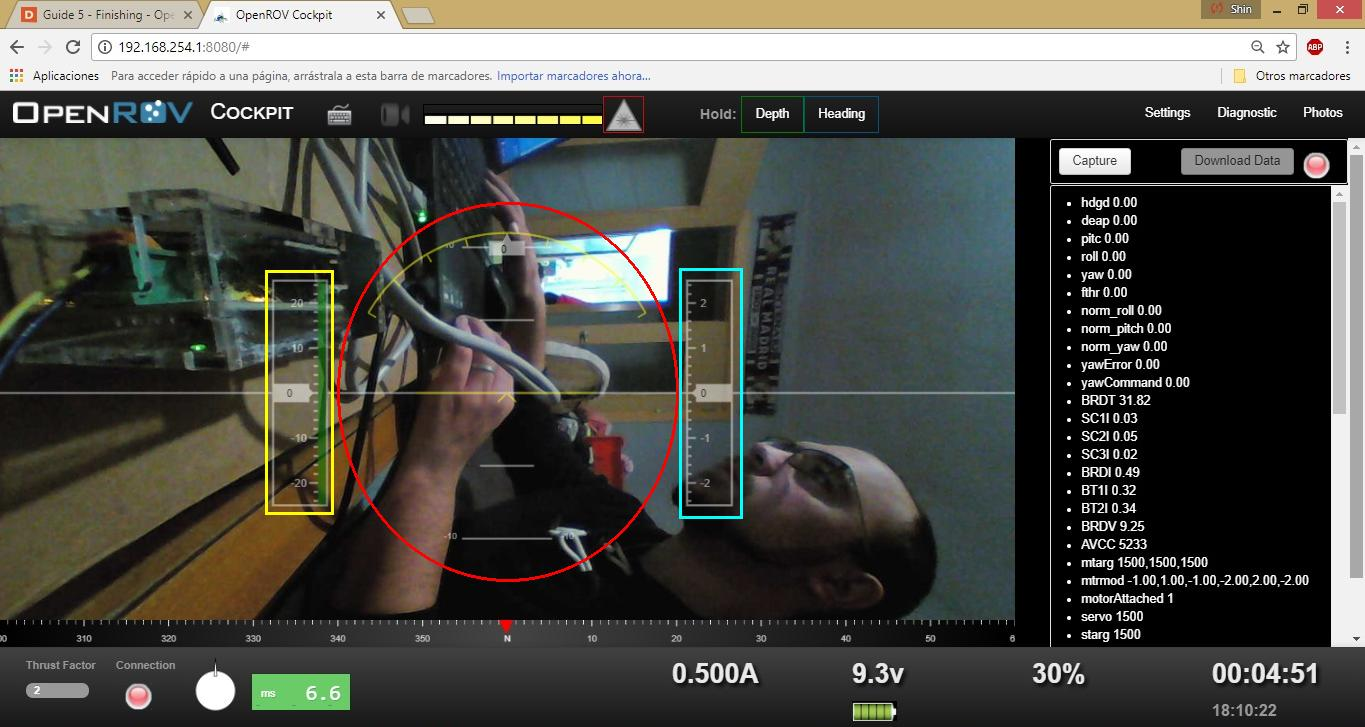
\includegraphics[width=15cm]{img/cap3/3_5/cockpit3_v2}
\end{center}
\caption{Cockpit (3)}
\label{fig:cockpit3}
\end{figure}
\begin{itemize}
\item[\textcolor{yellow}{\textbullet}]Fuerza de empuje del motor.
\item[\textcolor{red}{\textbullet}]Horizonte artificial.
\item[\textcolor{blue}{\textbullet}]Profundidad.
\end{itemize}

\begin{figure} [hbtp]
\begin{center}
  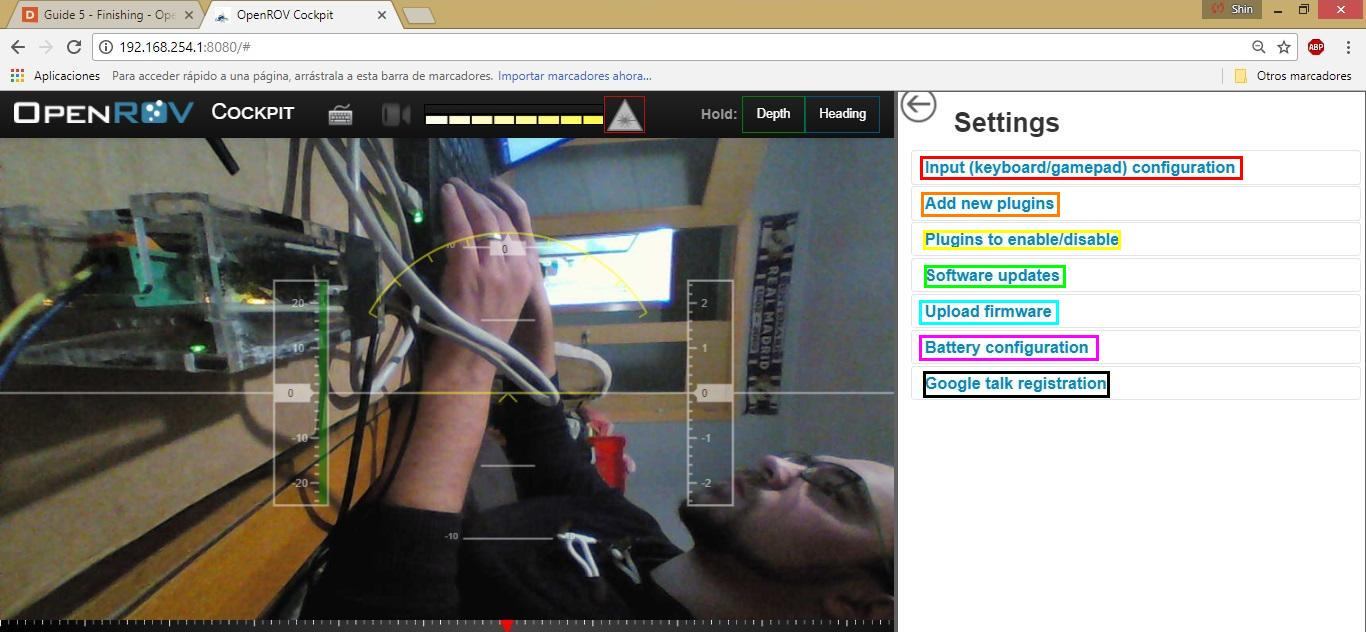
\includegraphics[width=15cm]{img/cap3/3_5/setting}
\end{center}
\caption{Ajustes}
\label{fig:settting}
\end{figure}
\newpage
Panel de configuración:
\begin{itemize}
 \item[\textcolor{red}{\textbullet}] Configuración de entrada: para personalizar los comandos de uso del robot.
 \item[\textcolor{orange}{\textbullet}] Agregar nuevos complementos.
 \item[\textcolor{yellow}{\textbullet}] Habilitar/deshabilitar complementos: activa y desactiva los complementos agregados en el punto anterior.
 \item[\textcolor{green}{\textbullet}] Actualización de software.
 \item[\textcolor{blue}{\textbullet}] Actualización del firmware.
 \item[\textcolor{purple}{\textbullet}] Configuración de la batería: Se establece el voltaje mínimo y máximo de la batería.
 \item[\textcolor{black}{\textbullet}] Registro de Google Talk: Permite el acceso a las de redes sociales de la web.
 \end{itemize}

\begin{figure} [hbtp]
\begin{center}
  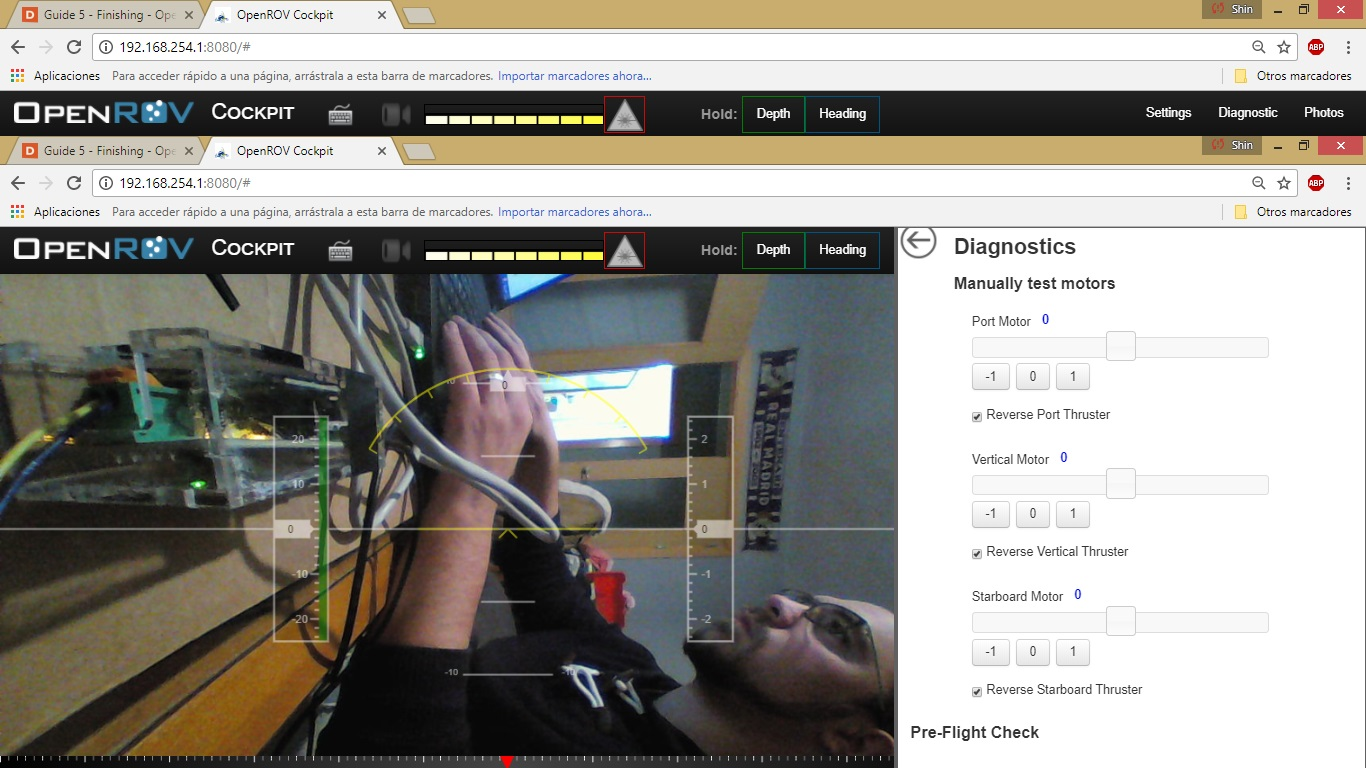
\includegraphics[width=15cm]{img/cap3/3_5/diagnostico}
\end{center}
\caption{Diagnóstico}
\label{fig:diagnostico}
\end{figure}

Panel de diagnósticos:
\begin{itemize}
 \item Verificación manual los motores.
 \item Si hay un error con la dirección de los motores se puede invertir desde este panel.
 \item Pre-Flight Check, es el marcador de la posición actual.
\end{itemize}

\begin{figure} [hbtp]
\begin{center}
  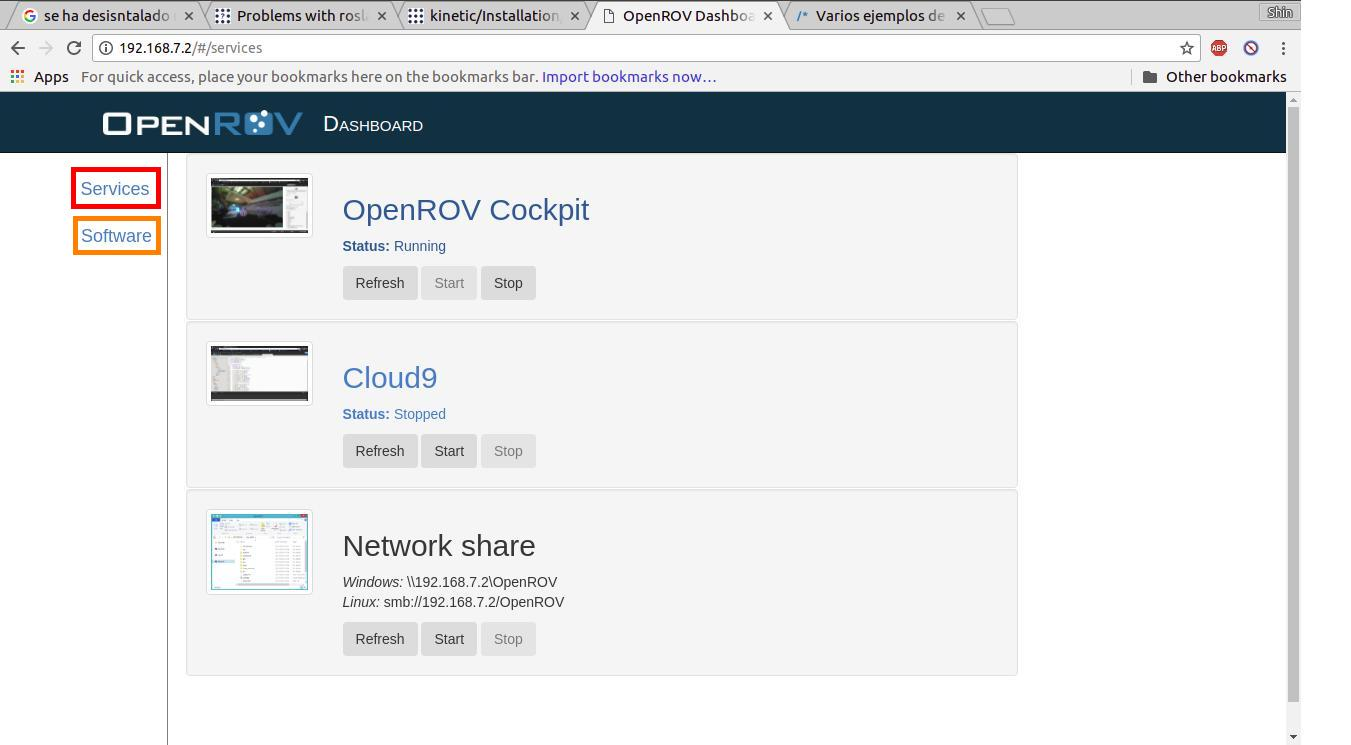
\includegraphics[width=15cm]{img/cap3/3_5/services}
\end{center}
\caption{Servicios}
\label{fig:services}
\end{figure}

El panel de configuración de OpenROV se encuentra en: 192.168.254.1.

Hay dos partes:
\begin{itemize}
\item[\textcolor{red}{\textbullet}]\textbf{Servicios}: Reinicia la web del ROV.
\item[\textcolor{orange}{\textbullet}]\textbf{Software}: Determina la versión del software y puede ejecutar la actualización del software del ROV.
\end{itemize}

\subsection{Mantenimiento}
\label{subsec:mantenimiento}

Para que la vida útil del robot sea lo más larga posible, se deben seguir unas ciertas pautas de mantenimiento.

\subsubsection{Enjuagar}
\label{subsubsec:enjuagar}
Una vez que hayamos utilizado el robot, tendremos que enjuagarlo en agua después de cada inmersión, para mantenerlo limpio y libre de desechos y minerales.
  
\subsubsection{Mantenimiento de los motores}
\label{subsubsec:mantenimiento}
Después de haber utilizado el robot en una inmersión, se debe limpiar los motores, ya que tienden a corroerse fácilmente. Se recomienda lubricarlos.

Los pasos que debemos seguir son los siguientes:
\begin{enumerate}
\item Enjuagar los motores en agua fría.
\item Secar los motores (es recomendable usar una pistola de aire comprimido).
\item Para finalizar el mantenimiento, lubricaremos los motores con un spray.
\end{enumerate}
Estos puntos deben hacerse antes y después de cada inmersión.
  
\subsubsection{Secado}
\label{subsubsec:secado}
Antes de guardar el OpenROV en su maletín, debemos asegurarnos de que no queda ninguna pieza mojada.
Para un mayor secado utilizaremos una pistola de aire comprimido y desmontaremos los tubos de las baterías y el tubo principal para cerciorarnos de que las baterías y la electrónica están secos.
  
\subsubsection{Carga de baterías}
\label{subsubsec:bateria}
El robot funciona con seis baterías, las cuales se cargarán a la vez, ya que se necesitan todas para el funcionamiento del robot.
\\Cada tubo lleva tres baterías. Si se intuye que alguna tiene un rendimiento inferior, se verificará utilizando un polímetro.
\\Es importante mantener las baterías secas y sin corrosión.

\subsection{Problemas}
\label{subsec:problemas}

Durante la vida útil del OpenROV pueden surgir ciertos imprevistos. A continuación, se detallan los problemas más comunes y cómo solucionarlos.
\begin{enumerate}
\item \textbf{Vaho} durante todo el proceso de sumersión.

El tubo principal puede empañarse tanto en la superficie (días soleados) como durante la sumersión.

Si el problema ha surgido en la superficie, retiraremos el tubo principal y lo limpiaremos con un paño. Si se empaña durante la inmersión, lo más recomendable es salir a la superficie y verificar que no existe ninguna fuga en el tubo principal.

La forma de solucionar el vaho es a través de los productos anti-vaho, además de cerciorarnos de que el tubo es estanco.

\item \textbf{Vídeo}.

Otro de los problemas más comunes es un corte o apagón en el vídeo que reproduce el robot en el fondo oceánico. 

Para evitar este fallo, es recomendable actualizar periódicamente la imagen del software en el BeagleBone.

\item \textbf{Control u otros problemas misceláneos}.

En las situaciones en las que el error provenga del control o fallos ajenos, el procedimiento a seguir es reiniciar el robot desenchufando el clable USB del PLC y volver a conectarlo.

\item \textbf{Pérdida aleatoria de energía de la batería}.

Si comprobamos que existen pérdidas de energía, primero comprobaremos que las baterías hacen contacto entre sí y que están colocadas de la forma correcta.

Si el fallo persiste, se verifica la potencia (alrededor de los 9V) a través de los pines correspondientes del conector DB-25.

Además, se puede comprobar cada batería individual para asegurarse de que tenga el voltaje correcto a través de un polímetro.

\begin{figure} [hbtp]
\begin{center}
  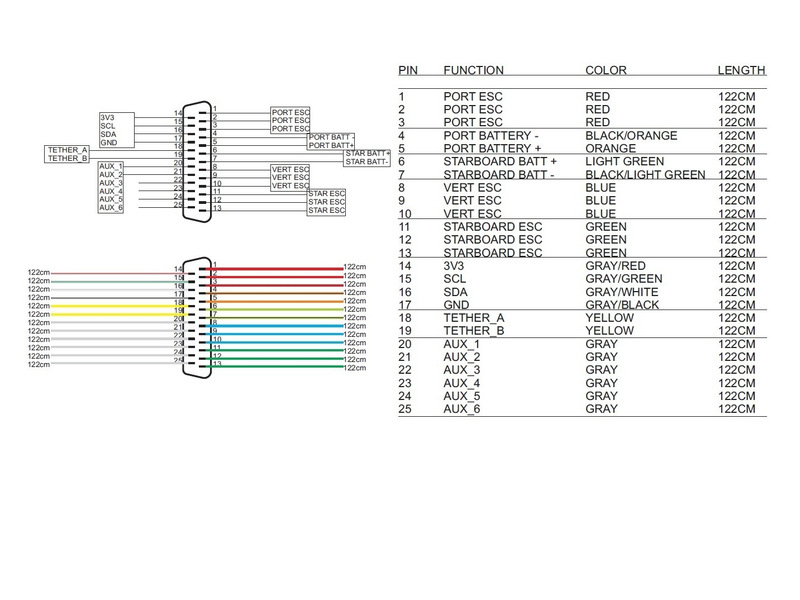
\includegraphics[width=12cm]{img/cap3/3_5/DB-25}
\end{center}
\caption{DB-25}
\label{fig:db25}
\end{figure}

\newpage

\item \textbf{Enredos}.

Fácilmente el robot puede quedar atrapado en el suelo oceánico por culpa de las algas u otros objetos o vegetales. Lo mejor es evitar pilotar el robot en un paisaje con una vegetación densa.

Si comprobamos que no se puede sacar el OpenROV por medio de los comandos, tiraremos de la correa hasta la superficie. Si aún así no podemos recuperar el robot, podemos cortar la correa e ir a buscarlo, ya que la correa puede volver a soldarse.

\item \textbf{Inundación del tubo principal}.

El mayor problema al que nos podemos enfrentar es que se inunde el tubo principal, que conllevaría al riesgo de perder el hardware del robot.

Primero, desconectaremos la alimentación del robot desenchufando el cable USB y seguidamente retiraremos las baterías.

Enjuagaremos los componentes electrónicos que se mojaron en el agua para eliminar los residuos del hardware, desmontaremos los componentes electrónicos y volveremos a enjuagar.

Secaremos bien cada una de las piezas de la electrónica. Lo más recomendable es usar una pistola de aire comprimido.

Para finalizar, colocaremos todos los componentes electrónicos afectados en un lugar seco. Lo mejor es usar una bolsa llena de arroz.

Cuando se vuelve a montar el robot, verificaremos que no exista corrosión. Si la hubiera, se intentará eliminar con un cepillo.
\end{enumerate}
